%!TEX TS-program = pdflatex
\documentclass[runningheads,envcountsame]{llncs}
%\documentclass[a4paper, cleveref]{lipics-v2021}
%
\usepackage[T1]{fontenc}
% T1 fonts will be used to generate the final print and online PDFs,
% so please use T1 fonts in your manuscript whenever possible.
% Other font encondings may result in incorrect characters.
%
\usepackage{graphicx}
\usepackage{tikz}
\usetikzlibrary{calc}

\usepackage{amsmath}
\usepackage{amssymb}

\usepackage{verbatim}
\usepackage[linesnumbered]{algorithm2e}

\spnewtheorem{claim*}[lemma]{Claim}{\itshape}{\normalfont}
\spnewtheorem*{cproof}{Proof of Claim}{\itshape}{\rmfamily}
%\newtheorem*{myclaim}{Claim}

%\newenvironment{claimproof}
%{\begin{cproof}
%}
%{\hfill$\blacksquare$
%\end{cproof}
%}

%\spnewtheorem{thm}{Theorem}{\bfseries}{\itshape}

\newenvironment{proof*}
{\begin{proof}
	}
	{\qed
\end{proof}}

\newcommand{\angl}[1]{\langle #1 \rangle}
\newcommand{\dom}[1]{\text{dom}(#1)}
\newcommand{\sem}[1]{\text{range}(#1)}
\newcommand{\ren}{\bigsqcup}
\newcommand{\su}{^{\$}}
\newcommand{\rk}{\text{rk}}
\def \<#1>{{\langle {#1} \rangle}}
\newcommand\lcop[1]{\left\lfloor{#1}\right\rfloor}
\newcommand\paras[1]{\mathsf{ps}(#1)}
\newcommand\he[1]{\mathsf{ht}(#1)}
\newcommand\comp[1]{\mathsf{comp}(#1)}
\newcommand\nop{\$}
\newcommand\pout{\mathit{pOut}}
\newcommand\tree[1]{\mathcal{T}_{#1}}
\newcommand\emp{\emptyset}
\newcommand\eps{\varepsilon}
\newcommand\ab{\allowbreak}
\newcommand\rhs{\mathit{rhs}}
\newcommand\ot{\leftarrow}
\newcommand\sos[1]{[\![#1]\!]}
\newcommand{\QY}{\Theta}

\newcommand{\N}{\mathbb{N}}
\newcommand\SC{\mathfrak{S\!C}}
\newcommand\MTTR{\text{MTT}^\text{R}}

\title{Deciding Linear Height and Linear Size-to-Height Increase of
  Macro Tree Transducers}
%TODO Please add
%
\titlerunning{Deciding Linear Increase Properties of Macro Tree Transducers}
% If the paper title is too long for the running head, you can set
% an abbreviated paper title here
%
%\author{Paul Gallot}{Universit\"at Bremen, Germany}{}{}{}
%\author{Sebastian Maneth}{Universit\"at Bremen, Germany}{}{}{}
%\author{Keisuke Nakano}{Tohoku University, Sendai, Japan}{}{}{}
%\author{Charles Peyrat}{ENS Paris-Saclay, France}{}{}{}
%\authorrunning{P. Gallot, S. Maneth, K. Nakano, and C. Peyrat}{}{}{}

\author{Paul Gallot\inst{1}\and Sebastian Maneth\inst{1} \and Keisuke Nakano\inst{2} \and Charles Peyrat\inst{3} }{}{}{}{}
% First names are abbreviated in the running head.
% If there are more than two authors, 'et al.' is used.
%
\institute{Universit\"at Bremen, Germany \and Tohoku University, Sendai, Japan\and ENS Paris-Saclay, France }

%\Copyright{CC-BY}%mandatory, please use full first names. LIPIcs license is "CC-BY";  http://creativecommons.org/licenses/by/3.0/
%\ccsdesc[500]{Theory of computation~Transducers} %TODO mandatory: Please choose ACM 2012 classifications from https://dl.acm.org/ccs/ccs_flat.cfm 
%\keywords{automata, formal language theory, macro tree transducer, normal form}%mandatory

\begin{document}

\maketitle


%TODO mandatory: add short abstract of the document
\begin{abstract}
We present a novel normal form for (total deterministic) macro tree transducers (mtts),
called ``depth proper normal form''. If an mtt is in this normal form,
then it is guaranteed that each parameter of each state 
%of the mtt 
appears 
at arbitrary depths in the output trees of that state. Intuitively, if some parameter
only appears at certain bounded depths in the output trees of a state, then
this parameter can be eliminated by in-lining the corresponding output paths at
each call site of that state. We use regular look-ahead in order to determine
which of the paths should be in-lined. As a consequence of changing the look-ahead,
a parameter that was previously appearing at unbounded depths,
may be appearing at bounded depths for some new look-ahead; for this reason, our
construction has to be iterated 
%in order 
to obtain an mtt in depth-normal form.
Using the normal form, we can decide whether the translation of an mtt
has linear height increase or has linear size-to-height increase.
\end{abstract}

\input{ICALP_introduction}
\section{Preliminaries}
In this section, we describe the necessary background for automated planning and the significance of the International Planning Competition. 

% \subsection{Ontology}
% A formal ontology is typically represented as a set of concepts, relations, and axioms. A concept represents a set of objects or entities that share common properties, while a relation represents a connection or association between two or more concepts. Axioms are statements that define the relationships between concepts and relations. It is a formal representation of knowledge that is designed to facilitate automated reasoning and information processing. It acts as a structured vocabulary that describes a domain and promotes interoperability, data integration, and communication between humans and machines. Formally, an ontology $O$ can be represented as a tuple $(C, R, A)$, where $C$ is the set of concepts, $R$ is the set of relations, and $A$ is the set of axioms. Each concept \textit{c} $\in$ $C$ can be represented as a set of attributes, denoted as $Att(c)$. Similarly, each relation \textit{r} $\in$ $R$ can be represented as a set of attributes, denoted as $Att(r)$.

% Ontology is a branch of philosophy that deals with the nature of existence and being. In the field of computer science, however, ontology refers to a formal representation of knowledge that is designed to facilitate automated reasoning and information processing. It is a structured vocabulary that describes a domain and promotes interoperability, data integration, and communication between humans and machines. Various tools and methodologies, including Protege and ontology editors, are available for ontology creation. Ontologies are increasingly important in artificial intelligence, knowledge engineering, and the semantic web, and researchers are exploring their potential in diverse domains and applications.

% Figure environment removed

\subsection{Automated Planning}

Automated planning, also known as AI planning, is the process of finding a sequence of actions that will transform an initial state of the world into a desired goal state \cite{ghallab2004automated}. It involves constructing a plan or a sequence of actions that will achieve a specified objective while respecting any constraints or limitations that may be present. Formally, automated planning can be defined as a tuple $(S, A, T, I, G)$, where:
\begin{itemize}
    \item $S$ is the set of possible states of the world
    \item $A$ is the set of possible actions that can be taken
    \item $T$ is the transition function that describes the effects of taking an action on the current state of the world
    \item $I$ is the initial state of the world
    \item $G$ is the desired goal state
\end{itemize}
Using this notation, the problem of automated planning can be framed as finding a sequence of actions $\prec a_1, a_2, ..., a_k\succ$ that will transform the initial state $I$ into the goal state $G$, while respecting any constraints or limitations on the actions. 
 % In automated planning, 
 A problem is defined in terms of a domain and a problem instance. The domain defines the possible actions that can be taken and the effects of each action, while the problem instance specifies the initial state of the world and the desired goal state. 
Various techniques can be used to solve the planning problem, such as search algorithms, constraint-based reasoning, and optimization methods. These techniques involve exploring the space of possible plans and selecting the one that satisfies the objective and any constraints. Figure \ref{fig:planning_bw} illustrates an automated planning scenario for the blocksworld domain, where an initial state can be transformed into a goal state by executing a sequence of actions.

% \noindent \textbf{Attributes modeled about a domain.}
%   %\noindent \textbf{Attributes modeled in a domain file}
%  \begin{enumerate}
%      \item \textbf{Requirements:} A list of requirements that the planner must satisfy in order to solve the domain. Requirements include durative actions, conditional effects, or negative preconditions. For example, in blocksworld domain with types involved, one of the requirements is \emph{typing}.
%     \item \textbf{Predicates:} Predicates are fundamental elements in the planning domain that define the properties of the world. They are used to describe the initial and goal states, as well as the preconditions and effects of actions. Predicates are usually defined as logical expressions over a set of variables, where each variable can take on a finite number of values. In the context of planning, predicates are typically used to represent facts about the world that can be true or false, such as the location of an object or the status of a machine. For example, in blocksworld domain, the predicate \verb|(on b1 b2)| could indicate that block 'b2' is on top of block 'b1'.
%      \item \textbf{Actions:} Actions are the basic units of change in the planning domain. They represent atomic operations that can be performed to transform the world from one state to another. Each action has a name, a set of parameters, preconditions that must be satisfied before the action can be executed, and effects that describe the changes that the action makes to the world. Actions can be used to model a wide variety of operations, ranging from simple movements or transformations to complex processes such as planning or decision-making. For example, in blocksworld domain, the action \verb|unstack b2 b1| can be used to unstack block 'b2' from block 'b1'. 
     
%      \item \textbf{Preconditions:} Preconditions are the conditions that must be true before an action can be executed. They are usually defined using predicates and can involve multiple variables. Preconditions can also be negative, which means that a certain condition must not be true for an action to be executed. In planning, preconditions ensure that actions are only executed when the necessary conditions have been met, such as ensuring that a machine is turned off before it is serviced. For example, in blocksworld domain, the action \verb|unstack b2 b1| has a precondition of \verb|(on b1 b2)|, meaning that for the action to be valid, the block 'b2' should be on top of block 'b1'.
     
%      \item \textbf{Effects:} Effects describe the changes that an action makes to the world. They are usually defined using predicates and can involve multiple variables. Effects can be positive, which means that a certain condition becomes true after the action is executed, or negative, which means that a certain condition becomes false after the action is executed. In the context of planning, effects are used to model the changes that result from executing an action, such as moving an object from one location to another or turning a machine on. For example, in blocksworld domain, when the action \verb|unstack b2 b1| is executed, one of its effect is \verb|(not (on b1 b2))|, indicating that block 'b2' is no longer on top of block 'b1'.
     
%      \item \textbf{Constants:} Constants are values that are fixed and do not change during the execution of the planning problem. They are used to represent objects or entities in the world that have a fixed value, such as the speed limit on a road. Constants can be used to simplify the planning problem by reducing the number of variables that need to be considered and by providing a fixed set of values that can be used in predicates and actions. For example, in blocksworld domain, the constant \emph{table} could represent the surface on which the blocks are initially placed.
     
%      \item \textbf{Types:} Types are used to classify objects or entities in the world based on their attributes or properties. They are used to define the domain of values that a variable can take on and can be used to constrain the values that are assigned to variables. In the context of planning, types are typically used to group related objects or entities together, such as cars or bicycles, and to specify the properties that are common to all members of a type, such as their color or size. For example, in blocksworld domain with types involved, one can represent the predicate as \verb|(on ?x - block ?y - block)| stating that the parameters in the predicate are of type \emph{block}.

%  \end{enumerate}


% ######### Shorter version for AI Planning preliminaries
% \subsection{Automated Planning}

% Automated planning, also known as AI planning, finds actions transforming an initial world state into a goal state \cite{ghallab2004automated}. It involves creating a plan, respecting constraints, defined as $(S, A, T, I, G)$ where $S$ is the world states set, $A$ is the actions set, $T$ is the state transition function, $I$ is the initial state, and $G$ is the goal state. The challenge is to find actions $\prec a_1, a_2, ..., a_k\succ$ converting $I$ to $G$ under constraints. 

% A problem has a domain (defining actions and effects) and an instance (specifying initial and goal states). Various techniques can be used to solve the planning problem, such as search algorithms, constraint-based reasoning, and optimization methods. These techniques involve exploring the space of possible plans and selecting the one that satisfies the objective and any constraints. Figure \ref{fig:planning_bw} illustrates an automated planning scenario for the blocksworld domain, where an initial state can be transformed into a goal state by executing a sequence of actions.

\noindent \textbf{Attributes modeled about a domain.}
 \begin{enumerate}
     \item \textbf{Requirements:} A list of requirements that the planner must satisfy to solve the given domain, e.g., \emph{typing} in blocksworld with types.
     \item \textbf{Predicates:} Define world properties, e.g., \verb|(on b1 b2)| in blocksworld.
     \item \textbf{Actions:} Units of change with preconditions and effects, e.g., \verb|unstack b2 b1| in blocksworld.
     \item \textbf{Preconditions:} Conditions for action execution, e.g., \verb|(on b1 b2)| for \\ \verb|unstack b2 b1|.
     \item \textbf{Effects:} Post-action world changes, e.g., \verb|(not (on b1 b2))| after \\ \verb|unstack b2 b1|.
     \item \textbf{Constants:} Fixed values, e.g., \emph{table} in blocksworld.
     \item \textbf{Types:} Classifications based on attributes, e.g., \\ \verb|(on ?x - block ?y - block)| in typed blocksworld.
 \end{enumerate}

\noindent \textbf{Attributes modeled about a problem instance from a domain.}
\begin{enumerate}
    \item \textbf{Name:} The name of the planning problem.
    \item \textbf{Domain:} The name of the planning domain that the problem belongs to.
    \item \textbf{Objects:} A list of objects that are present in the planning problem. Objects are typically defined in terms of their type and name. In the example shown in Figure \ref{fig:planning_bw}, objects are b1, b2, and b3.
    \item \textbf{Initial State:} A description of the initial state of the world, including the values of all relevant predicates. Figure \ref{fig:planning_bw} represents an example initial state.
    \item \textbf{Goal State:} A description of the desired goal state of the world, including the values of all relevant predicates. Figure \ref{fig:planning_bw} represents an example goal state.
\end{enumerate}

% \vspace{2cm}
\subsection{International Planning Competition (IPC)}

% IPC serves as a significant means of assessing and comparing various planning systems. By presenting new planners and benchmark problems each year, the competitions aim to stimulate the advancement of new planning methodologies and reflect current trends and challenges in the field. The competition comprises multiple tracks, each covering various planning problems such as classical, temporal, and probabilistic planning. These tracks include benchmark problems that evaluate the performance of planners concerning parameters such as plan quality, plan length, and run time. The results of these competitions provide insights into the current state-of-the-art in planning and help identify the strengths and weaknesses of different planning systems. IPC can serve as an excellent starting point for building a planning-related ontology as the benchmark problems used in these competitions can provide a comprehensive overview of the domain and the types of problems that planners need to solve. 

IPC is pivotal for evaluating and contrasting planning systems. Introducing new planners and benchmarks, it promotes innovative planning methodologies and reflects the field's evolving challenges. The competition has multiple tracks, such as classical and probabilistic planning, with benchmarks assessing plan quality, length, and run time. IPC results offer a glimpse into the latest in planning, highlighting system pros and cons. The benchmarks from IPC are ideal for crafting a planning-related ontology, encapsulating the domain's breadth and planners' challenges.

%!TEX root = main.tex
\section{Depth Proper Normal Form}

The depth proper normal form requires that each parameter of
each state $q$ occurs at unbounded depth in the output trees of that state 
(for each given look-ahead state $p$ such that $(q,p)$ is reachable).
Formally, let $q$ be a state of rank $m\geq 1$, $j\in[m]$, and
$p\in P$. 
If $(q,p)$ is reachable, then 
for every natural number $n$ there must exist an input tree $s_n \in L_p$ such that
$y_j$ occurs at depth $>n$ in the tree $M_q(s_n)$.
Conversely, we say that parameter $y_j$ is \emph{depth-bounded} for $q$ and $p$ 
if there exists an $n$ for which no such input tree $s_n \in L_p$ exists;
more generally, we say that $Z\subseteq Y_m$ is
\emph{depth-bounded} for $q$ and $p$, if each $y\in Z$ is depth-bounded for $q$ and $p$.

If $Z$ is depth-bounded for $q$ and $p$, then there are only finitely many output paths
in the trees in $M_q(L_p)$ under which the parameters from $Z$ occur.
The \emph{$Z$-skeleton} of an arbitrary tree $t$ is obtained from $t$
by replacing each top-most node $u$ such that $t/u$ does not contain any
occurrence of a parameter from $Z$ by some symbol. 
Clearly, $Z$ is depth-bounded for $q$ and $p$ if and only if the $Z$-skeleta of
all trees in $M_q(L_p)$ form a finite set.

Let $\Delta$ be an arbitrary ranked alphabet, $m\geq 1$, 
$t\in T_\Delta(Y_m)$, and $Z\subseteq Y_m$.
Let us write \(\paras{t}\subseteq{Y_m}\) for the set of parameters 
occurring in $t$.
Let us now be more specific as to which symbols replace the top-most nodes $u$
of $t$ such that $\paras{t/u}\cap Z=\emptyset$. Since in our construction later
we will want to obtain a transducer that is nondeleting, it will be helpful
to know which parameters appear in a given deleted tree. Therefore we replace
such nodes $u$ by the set $\paras{t/u}$. 
We denote by $\lcop{t}_Z$ the $Z$-skeleton of $t$ and define it inductively as follows
(where $\delta\in\Delta$):
\begin{align*}
\lcop{t}_Z &= 
\begin{cases}
t &
\text{if \(t\in Z\)}
\\
\delta(\lcop{t_1}_Z,\dots,\lcop{t_n}_Z) &
\text{if \(\paras{t}\cap Z\ne\emptyset\) and \(t = \delta(t_1,\dots,t_n)\)}
\\
\paras{t} & \text{if \(\paras{t}\cap Z = \emptyset\)}.
\end{cases}
\end{align*}

The definition of $\lcop{t}_Z$ is extended to sets $L$ of trees
as $\lcop{L}_Z=\{\lcop{t}_Z\mid t\in L\}$.
We call \emph{$Y$-nodes} the nodes $u$ in $V(\lcop{t}_Z)$ such 
that $\lcop{t}_Z/u=Z'\subseteq Y_m$. We denote by 
$\mathcal{U}(\lcop{t}_Z)$ the set of $Y$-nodes on $\lcop{t}_Z$. 
The notion of parameters in a tree naturally extends to $Z$-skeleta with, 
for a $Y$-node labeled $Z'$: $\paras{Z'} = Z'$. 
The proof of the next lemma is straightforward by induction on $t$
(see the Appendix).

\begin{lemma}\label{lm:nd}
Let $\Delta$ be a ranked alphabet, $m\geq 1$, $Z\subseteq Y_m$, and
$t\in T_\Delta(Y_m)$.
(1)~$t=\lcop{t}_Z[u\leftarrow t/u\mid u\in\mathcal{U}(\lcop{t}_Z)]$.
(2)~$\paras{\lcop{t}_Z} = \paras{t}$. 
%(3)~If $y\in Y_m$ occurs in $t$, then 
%there exists a leaf $u\in V(\lcop{t}_Z)$
%such that either $\lcop{t}_Z/u=y$ or 
%$\lcop{t}_Z/u=Z'\subseteq Y_m$ and $y\in Z'$.
\end{lemma}

%%Sebastian's version:
%The proof is by induction on the structure of $t$.
%Let us denote the substitution $[u\leftarrow t/u\mid u\in\mathcal{U}(\lcop{t}_Z)]$
%by $[t]$.
%%
%We first consider $t=y\in Y$. There are two cases.
%
%Case 1: $y\in Z$. Then $\mathcal{U}(\lcop{t}_Z)=\emptyset$.
%Hence $\lcop{t}_Z[t]=\lcop{y}_Z$. The latter equals $y=t$ by 
%the definition of $\lcop{.}_Z$. Thus~(1)~holds and~(2)~holds for $u=\epsilon$.
%
%Case 2: $y\not\in Z$. Then $\mathcal{U}(\lcop{t}_Z)=\{ \epsilon \}$ and hence
%$\lcop{t}_Z[t] = \lcop{t}_Z[\epsilon\leftarrow t/\epsilon = t] = t$ which proves~(1).
%Moreover, $\lcop{t}_Z=\{y_j\}$ by the definition of $\lcop{.}_Z$,
%i.e., again~(2)~holds for $u=\varepsilon$.
%
%Now consider $t=\delta(t_1,\dots,t_n)$, $\delta\in\Delta^{(n)}$, $n\geq 0$,
%and $t_1,\dots, t_n\in T_\Delta(Y_m)$.
%To show~(1) we obtain from the definition $\lcop{t}_Z$ that
%\[
%\lcop{t}_Z[t]=\delta(\lcop{t_1}_Z,\dots,\lcop{t_n}_Z)[t]
%= \delta(\lcop{t_1}_Z[t_1],\dots,\lcop{t_n}_Z[t_n]),
%\]
%where for $i\in[n]$, $[t_i]$ denotes the substitution
%$[u\leftarrow t_i/u\mid u\in\mathcal{U}(\lcop{t_i}_Z)]$.
%By induction the latter equals $\delta(t_1,\dots,t_n)=t$.
%To show~(2) we assume that $y_j$ occurs in $t$ for some $j\in[m]$.
%Thus, $n\geq 1$ and there exists an $i\in[n]$
%such that $y_j$ occurs in $t_i$.
%By the induction for Statement~(2), there exists a leaf $u$ of $t_i$ such that 
%the Statement~(2) holds (for $u$ and $t_i$), and therefore Statement~(2) holds
%for $iu$ and $t$.
%\end{proof}

Finally, we define depth properness for mtts with look-ahead. 

\begin{definition} \label{df_depth_proper}
The mttr $M=(Q,P,\Sigma,\Delta,q_0,R,h)$ is in \emph{depth proper normal form}
(or, synonymously, $M$ is \emph{depth proper})
if for every $q\in Q^{(m)}$, $m\geq 1$, and $p\in P$ it holds that
if $(q,p)$ is reachable, then  
$\lcop{M_q(L_p)}_{\{y_j\}}$ is infinite for all $j\in[m]$.
\end{definition}

From now on we will want to make use of the following definitions:
\[
\begin{array}{lcl}
F_p &=& \{ q\in Q^{(m)}\mid \exists j\in[m], \lcop{M_q(L_p)}_{\{y_j\}}
\text{ is finite}\}\\
Y(q,p) &=& \{ y_j\mid j\in[\text{rank}_Q(q)]\text{ such that }
\lcop{M_q(L_p)}_{\{y_j\}}\text{ is finite}\}
\end{array}
\]

It should be clear that $\lcop{M_q(L_p)}_{Y(q,p)}$ is finite for every $q$ and $p$,
as stated in the next lemma (the proof is in the Appendix).

\begin{lemma}\label{lm:lcop_finite}
Let $M$ be an mtt, $q$ a state of $M$, and $p$ a look-ahead state of $M$
such that $Y(q,p)\not=\emptyset$.
Then $\lcop{M_q(L_p)}_{Y(q,p)}$ is finite.
\end{lemma}

\subsection{Construction of the Normal Form and Examples}
\label{sect:examples}

%\subsection{Formal Construction of the Depth Proper Normal Form}
%\label{sect:dp}

Let $M$ be an mttr as before. 
We assume that $M$ is nondeleting (which is justified by 
Proposition~\ref{prop:nondeleting}).
The idea of the construction is as follows.
First, we determine all reachable pairs $(q,p)$ 
such that $Y(q,p)\not=\emptyset$.
Let $(q,p)$ be such a pair and let $Z=Y(q,p)$.
An occurrence of $\<q,x_i>$ in a right-hand side
$\text{rhs}_M(q',\sigma,\< p_1,\dots,p_k>)$ such that $p_i=p$ is
called a \emph{$(q,p)$-call}. Our aim is to replace each $(q,p)$-call
by an appropriate tree from $\lcop{M_q(L_p)}_Z$. Just which tree is
the appropriate one will be determined by regular look-ahead. 
Moreover, such trees should be modified not to contain leaf nodes 
labeled by subsets of $Y$: such nodes will be replaced by 
calls of new ``helper states''. 

%We now present the formal construction of the transducer $\pi(M)$.
%Note that in general, $\pi(M)$ is \emph{not} depth proper yet, but
%the construction needs to be iterated several times (cf. the examples in
%Section~\ref{sect:examples}).

\begin{definition}
\label{df:pi}
Let $M=(Q,P,\Sigma,\Delta,q_0,R,h)$ be a nondeleting mttr
that is not depth proper.
We construct the new mttr
$\pi(M)=(Q\cup H,P',\Sigma,\Delta,q_0,R',h')$.
% The sets $H$ and $P'$ are defined as follows.
For every 
$q\in Q^{(m)}$, $m\geq 1$, and $p\in P$ such that $Y(q,p)\not=\emptyset$,
$H$ contains the following set of helper states:
\[
\{ [q,p,t,u]^{(|U|)}\mid 
t\in \lcop{M_q(L_p)}_{Y(q,p)}, 
u\in V(t),
t/u=U\subseteq Y_m \}
\]
and $P'$ contains $(p,\varphi)$ for any
function $\varphi$ that assigns to each $q\in F_p$ 
a tree in $\lcop{M_q(L_p)}_{Y(q,p)}$.
%
Observe that $H$ and $P'$ are well defined, because
$\lcop{M_q(L_p)}_{Y(q,p)}$ is finite by Lemma~\ref{lm:lcop_finite}. 
%
Note that $|U|\leq |Y_m \setminus Y(q,p)|$; since $Y(q,p)$ is non-empty this implies that
the rank of each helper state is at most $(r-1)$, where $r$ is the maximal
rank of the states in $Q$. 

For every $q\in Q^{(m)}$, $m\geq 0$, 
$\sigma\in\Sigma^{(k)}$, $k\geq 0$, and 
$(p_1,\varphi_1),\dots,(p_k,\varphi_k)\in P'$ we let the rule
\[
\<q,\sigma(x_1:(p_1,\varphi_1),\dots,x_k:(p_i,\varphi_i)>(y_1,\dots,y_m)
\to\text{rhs}_M(q,\sigma,\<p_1,\dots,p_k>)[\![ . ]\!]
\]
be in $R'$, where the second-order tree substitution
$[\![ . ]\!]$ is defined as follows.
\begin{multline*}
[\![ . ]\!] = 
[\![\< q',x_i>\leftarrow \varphi_i(q')\big[
u\leftarrow [q',p_i,\varphi_i(q'),u](y_{j_1},\dots,y_{j_n})\mid \\
\varphi_i(q')/u=\{y_{j_1},\dots,y_{j_n}\},
j_1<\cdots <j_n\big] \mid q'\in F_{p_i}, i\in[k]
 ]\!].
\end{multline*}
We define $h_\sigma'((p_1,\varphi_1),\dots,(p_k,\varphi_k))=(p,\varphi)$
where $p=h_\sigma(p_1,\dots,p_k)$ and, using special second-order substitution 
from Definition~\ref{def:meta-skeleta}, for every $q\in F_p$,  
\[
\varphi(q)=
\lcop{
\text{rhs}_M(q,\sigma,\<p_1,\dots,p_k>)
[\![\< q',x_i>\leftarrow \varphi_i(q')\mid q'\in F_{p_i}, i\in[k]]\!]\su
}_{Y(q,p)}.
\]
%
For every helper state $[q,p,t,u]\in H^{(n)}$, $n\geq 0$,
$\sigma\in\Sigma^{(k)}$, $k\geq 0$, and 
$(p_1,\varphi_1),\dots,$ $(p_k,\varphi_k)\in P'$ 
such that $h_\sigma(p_1,\dots,p_k)=p$
we let the rule
\[
\<[q,p,t,u](\sigma(x_1:(p_1,\varphi_1),\dots,x_k:(p_k,\varphi_k))>(y_1,\dots,y_n)
\to \xi/u[y_{j_\nu}\leftarrow y_\nu\mid\nu\in[n]]
\]
be in $R'$ where
$t/u=\{y_{j_1},\dots,y_{j_n}\}$,
$j_1<\cdots <j_n$,
$\xi=\text{rhs}_M(q,\sigma,\<p_1,\dots,p_k>)[\![ . ]\!]$, and
$[\![ . ]\!]$ is the substitution from above.
\end{definition}

%We present two examples to show how a depth proper mttr is obtained.

\newcommand\qid{q_{\mathrm{id}}}

We now show how the depth proper normal form is achieved using
an example. An additional example (which makes more interesting use of
helper states) can be found in the Appendix. 
%
%Next we shall show a more complex example where
%a set of \(Z\)-skeleta is not singleton and 
%a $Y$-node of a \(Z\)-skeleton is not empty
%(and where the construction needs to be iterated).
%
Let \(M=(Q,\{p\},\Sigma,\Delta,q_0,R,h_0)\) 
with
\(Q=\{q_0^{(0)},q_1^{(1)},q_2^{(2)}\}\),
\(\Sigma=\{a^{(1)},b^{(1)},e^{(0)}\}\),
and \(\Delta=\{f^{(2)},g^{(1)},e^{(0)}\}\)
be an mttr 
where \((\Sigma,\{p\},h_0)\) with $L_p=T_\Sigma$
and \(R\) consists of these rules:
\begin{align*}
\<q_1, a(x)>(y_1) &\to \<q_2, x>(y_1, \<q_1,x>(y_1)) &
\<q_2, a(x)>(y_1,y_2) &\to f(y_1,\<q_1,x>(g(y_2)))
\\
\<q_1, b(x)>(y_1) &\to y_1 &
\<q_2, b(x)>(y_1,y_2) &\to f(y_2,y_1)
\\
\<q_1, e>(y_1) &\to g(y_1) &
\<q_2, e>(y_1,y_2) &\to f(y_2,y_1)
\end{align*}
We suppose that the \(q_0\)-rules are defined so that all states are reachable.
Now we have \(F_p=\{q_2\}\), \(Y(q_2,p)=\{y_1\}\), and 
\(\lcop{M_{q_2}(L_p)}_{\{y_1\}} = \{ t_1, t_2 \}\)
with \(t_1 = f(y_1,\{y_2\})\) and \(t_2=f(\{y_2\},y_1)\).
As before, we can rewrite \(q_2\)-calls with the skeleta,
but since there are two possibilities \(t_1\) and \(t_2\), 
we need to separate the rules according to the input using the look-ahead.
In general, \(F_p\) contains several states each of which may have multiple skeleta, 
so each look-ahead contains a finite map from \(F_p\) to skeleta.
Let \(\varphi_1=\{q_2\mapsto t_1\}\) and \(\varphi_2=\{q_2\mapsto t_2\}\) 
such that \(L_{p,\varphi_1}=\{a(s)\mid s\in\tree\Sigma\}\) and
\(L_{p,\varphi_2}=\{b(s)\mid s\in\tree\Sigma\}\cup\{e\}\).
The \((q_1,a)\)-rule containing a \(q_2\)-call is separated as
\begin{align*}
\<q_1,a(x:(p,\varphi_1))>(y_1) &\to f(y_1, \<[q_2,p,t_1,2],x>(\<q_1,x>(y_1))) \\
\<q_1,a(x:(p,\varphi_2))>(y_1) &\to f(\<[q_2,p,t_2,1],x>(\<q_1,x>(y_1)),y_1) 
\end{align*}
where \(\<[q_2,p,t_1,2],x>\) and \(\<[q_2,p,t_2,1],x>\) are helper states.
Each helper state has rank 1 
because the corresponding node in the skeleton is a $Y$-node of length 1.
The arguments of the call are inherited from
the arguments of the original \(q_2\)-call that occur in the sequence.
For example, \(\<[q_2,p,t_1,2],x>\) is called with \(\<q_1,x>(y_1)\)
since \(t_1\) has a $Y$-node \(\{y_2\}\) and 
the original \(q_2\)-call has \(\<q_1,x>(y_1)\) as the second argument.
The rules of these helper states are constructed from the original \(q_2\)-rule
with substitution (which causes nothing since no states in \(F_p\) are called)
and extracting a subtree at the $Y$-node, that is,
\[
\begin{array}{lcl}
\<[q_2,p,t_1,2], a(x:(p,\varphi))>(y_1) &\to& \<q_1,x>(g(y_1)) \\
\<[q_2,p,t_2,1], b(x:(p,\varphi))>(y_1) &\to& y_1 \\
\<[q_2,p,t_2,1], e>(y_1) &\to& y_1 
\end{array}
\]
where \(\varphi\in\{\varphi_1,\varphi_2\}\) and
we had to rename the parameter \(y_2\) into \(y_1\)
(because the helper states only refer to \(y_2\)).
Note that rules for \(([q_2,p,t_1,2],b)\), \(([q_2,p,t_1,2],e)\) and \(([q_2,p,t_2,1], a)\) 
do not have to be considered.
These rules are not referred because
the states are never called with the input symbols
due to their look-ahead.
For example, the \([q_2,p,t_1,2]\)-call occurs only 
in the \((q_1,a)\)-rule with \(x\in L_{p,\varphi_1}\)
in which the root symbol cannot be \(b\).
%They are not reachable because they are called with the specific look-ahead.

Thereby we have been able to remove every call of states in \(F_p\).
However, new improper states may be generated by the separation of rules 
because of the look-ahead introduction.
In fact, we have \(F_{p,\varphi_2}=\{q_1,q_2,[q_2,p,t_2,1]\}\) in the example above.
Since every \(q_2\)-call has already been removed in the previous step,
we have to apply the same technique again for the calls of 
\(q_1\) and \([q_2,p,t_2,1]\).
We have $Y(q_1,(p,\varphi_2))=\{y_1\}$ and 
$Y([q_2,p,t_2,1],(p,\varphi_2))=\{y_1\}$.
Moreover 
$\lcop{M'_{q_1}(L_{p,\varphi_2})}_{\{y_1\}}=\{y_1, g(y_1)\}$
and
$\lcop{M'_{[q_2,p,t_2,1]}(L_{p,\varphi_2})}_{\{y_1\}}=\{y_1\}$.

\iffalse
We have: \vspace{-2mm}
\begin{align*}
&Y(q_1,(p,\varphi_2))=\{y_1\}
&&\text{and}
&Y([q_2,p,t_2,1],(p,\varphi_2))=\{y_1\}, \\
&\lcop{M'_{q_1}(L_{p,\varphi_2})}_{\{y_1\}}=\{y_1, g(y_1)\}
&&\text{and}
&\lcop{M'_{[q_2,p,t_2,1]}(L_{p,\varphi_2})}_{\{y_1\}}=\{y_1\}\text.
\end{align*} \vspace{-5mm}
\fi


Look-ahead has to be introduced to determine which skeleton to output.
Two maps over \(F_{p,\varphi_2}\),
except for \(q_2\) whose call has already been removed,
are defined: 
\(\varphi_3=\{q_1\mapsto y_1, [q_2,p,t_2,1]\mapsto y_1\}\) and
\(\varphi_4=\{q_1\mapsto g(y_1), [q_2,p,t_2,1]\mapsto y_1\}\)
such that \(L_{p,\varphi_2,\varphi_3}=\{b(s)\in L_{p,\varphi_2}\mid s\in\tree\Sigma\}\) and
\(L_{p,\varphi_2,\varphi_3}=\{e\}\).
The \((q_1,a)\)- and \(([q_2,p,t_1,2],a)\)-rules with look-ahead \(\varphi_2\)
which contains a \(q_2\)-call 
are separated as follows:
\[
\begin{array}{lcl}
\<q_1, a(x:(p,\varphi_2,\varphi_3))>(y_1) &\!\to& f(y_1,y_1) \\
  \<[q_2,p,t_1,2], a(x:(p,\varphi_2,\varphi_3))>(y_1) &\!\to& g(y_1) \\
\<q_1, a(x:(p,\varphi_2,\varphi_4))>(y_1) &\!\to& f(g(y_1),y_1) \\
  \<[q_2,p,t_1,2], a(x:(p,\varphi_2,\varphi_4))>(y_1) &\!\to& g(g(y_1)) 
\end{array}
\]
The resulting  mttr is depth proper.

\iffalse
Let \(M=(\{q_0,q_1,q_2\},\{p\},\Sigma,\Delta,q_0,R,h_0)\) be an mttr 
where \((\Sigma,\{p\},h_0)\) is the trivial tree automaton on \(\tree\Sigma\)
and \(R\) consists of the rules:
\begin{align*}
&\<q_0, a(x)> \to g(\<q_1, x>(\<q_0, x>)) &
&\<q_0, b(x)> \to g(\<q_2, x>(e)) &
&\<q_0, e> \to e
\\
&\<q_1, a(x)>(y) \to f(y, y) &
&\<q_1, b(x)>(y) \to g(y) &
&\<q_1, e>(y) \to g(y) 
\\
&\<q_2, a(x)>(y) \to\<q_2,x>(g(y)) &
&\<q_2, b(x)>(y) \to f(y, \<q_0,x>) &
&\<q_2, e>(y) \to y
\end{align*}
where the look-ahead \(p\) is omitted.
Then we can find that \(M_{q_1}(L_p)=M_{q_1}(\tree\Sigma)\)
is finite, that is, \(M_{q_1}(L_p)=\{f(y,y),g(y)\}\),
and hence \(Y(q_1,p)=\{y\}\).
Let us call such states \emph{improper}.
Every call of the improper state \(q_1\) will be substituted (in a second-order fashion)
by either one of these trees, and which one is determined by look-ahead.
The look-ahead is given as a tree automaton \((P,\Sigma,h)\) with \(P=\{p_1,p_2\}\)
that satisfies
\(M_{q_1}(L_{p_1})=\{f(y,y)\}\), \(M_{q_1}(L_{p_2})=\{g(y)\}\),
and \(L_{p_1}\cup L_{p_2}=\tree\Sigma\).
Thereby the \(q_0\)-rule for \(a\) is split into two rules
\begin{align*}
\<q_0, a(x:p_1)> &\to g(f(\<q_0, x>, \<q_0, x>)) 
\\
\<q_0, a(x:p_2)> &\to g(g(\<q_0, x>)) 
\end{align*}
for \(\{y\}\)-skeleta \(f(y,y)\) and \(g(y)\), respectively,
and the other rules are split into two which have the same right-hand side as before.
Observe that there are no state call of \(q_1\).

Let \(M'\) be the obtained mttr.
Since \(L_{p_2}\) consists of two types of trees, 
either \(b(t)\) with \(t\in\tree\Sigma\) or \(e\),
we find that 
\(M_{q_2}(L_{p_2})=\{y\}\cup\{f(y,t)\mid t\in\tree\Delta\}\),
thus \(\lcop{M_{q_2}(L_{p_2})}_{\{y\}}=\{y, f(y,\emp)\}\) is finite.
In a way similar to the above,
we remove all \(q_2\)-calls for look-ahead \(p_2\)
by replacing them either by \(y\) or by \(f(y, t')\)
where look-ahead determines which one to be used.
The tree \(t'\) is constructed according to the original rules.
The refined look-ahead automaton is given by \((P\times P',\Sigma,h'')\)
with \(P'=\{p'_1,p'_2\}\)
that satisfies 
\(\lcop{M_{q_2}(L_{(p_2,p'_1)})}_{\{y\}} =\{y\}\),
\(\lcop{M_{q_2}(L_{(p_2,p'_2)})}_{\{y\}} = \{ f(y,\emp) \}\), 
\(L_{(p_2,p'_1)}\cup L_{(p_2,p'_2)}=L_{p_2}\).
Every rule of \(M'\) is split into two again
where the set of look-ahead states becomes \(P\times P'\).
The original \((q_0,b)\)-rule and \((q_2,a)\)-rule with look-ahead \(p_2\)
containing \(q_2\)-calls
will be split into different new rules:
\begin{align*}
\<q_0, b(x:(p_2,p'_1))> &\to g(e)
\\
\<q_0, b(x:(p_2,p'_2))> &\to g(f(e,\<[q_2,p_2,f(y,\emptyset),2],x>))
\\
\<q_2, a(x:(p_2,p'_1))>(y) &\to g(y)
\\
\<q_2, a(x:(p_2,p'_2))>(y) &\to f(g(y),\<[q_2,p_2,f(y,\emptyset),2],x>)
\end{align*}
where the first and the third rules are obtained as done in the previous step
using the \(\{y\}\)-skeleton \(y\)
while the other two rules are constructed not only by replacing the \(q_2\)-call
with the \(\{y\}\)-skeleton \( f(y,\emptyset) \) but also
by using the \emph{helper state} \([q_2,p_2,f(y,\emptyset),2]\)
to compute a concrete output tree at the node of \(\emptyset\).
The helper state plays a role of waiting for the time 
when it is able to give the output tree.
In general,
a helper state call \(\<[q,p,t,u]^{(|t/u|)},x>\) for \(x\in L_p\) is expected to
compute a subtree at \(u\) of \(M_q(x)\) of the form \(t\in\lcop{M_q(L_p)}_Z\)
where \(t/u\subseteq Y_{\rk(q)}\setminus Z\),
and hence the rules of the helper state are defined by the original \(q\)-rules
with traversing its right-hand side according to the path \(u\).
For the current example, from the original \((q_2,b)\)-rules, we obtain
\begin{align*}
\<[q_2,p_2,f(y,\emptyset),2],b(x:(p_i,p'_j))> &\to \<q_0,x> 
\end{align*}
for all \(i,j\in\{1,2\}\) such that \(h''_{b}((p_i,p'_j)) = (p_2,p'_2)\).
The other rules of \([q_2,p_2,\ab f(y,\emptyset),2]\) can be arbitrarily defined
because their inputs are not in \(L_{(p_2,p'_2)}\), so that they are not reachable.
Then we find the state \(q_2\) becomes improper
for \(L_{(p_1,p'_1)}\) and \(L_{(p_1,p'_2)}\)
where 
\(\lcop{M_{q_2}(L_{(p_1,p'_i)})}_{\{y\}}=\{g(y), f(g(y),\emptyset)\}\) with \(i=1,2\).
This procedure terminates as we will show later.

We shall show another example to illustrate how the helper states work.
Let \(M=(\{q_0,q_1,q_2\},\{p\},\Sigma,\Delta,R,h_0)\) be an mttr
with the trivial look-ahead \((\Sigma,\{p\},h_0)\) and \(R\) consists of the rules:
\begin{align*}
&\<q_0, a(x)> \to \<q_1, x>(e) &
&\<q_0, e> \to e \\
&\<q_1, a(x)>(y) \to f(\<q_2, x>(e,g(y,\<q_0,x>)),\<q_0,x>) &
&\<q_1, e>(y) \to f(g(e,g(y,e)),e) \\
&\<q_2, a(x)>(y_1,y_2) \to g(\<q_2,x>(g(y_1,e),e),y_2) &
&\<q_2, e>(y_1,y_2) \to g(y_1,y_2)
\end{align*}
Then we find that two states \(q_1\) and \(q_2\) are improper
since both
\(\lcop{M_{q_1}(L_p)}_{\{y\}}=\{f(g(\emp,g(y,\emp)),\emp)\}\)
and
\(\lcop{M_{q_2}(L_p)}_{\{y_2\}}=\{g(\{y_1\},y_2)\}\)
are finite.
We will remove every call of both improper states simultaneously.
%This example is more complex than the previous one
%because the finiteness of \(\lcop{M_{q_1}(L_p)}_{\{y\}}\) is found
%not only the \(q_1\)-rules but also the \(q_2\)-rules.
Let \(t_1=f(g(\emp,g(y,\emp)),\emp)\) and \(t_2=g(\{y_1\},y_2)\)
be the \(\{y\}\)-skeleton for the state \(q_1\)
and the \(\{y_1\}\)-skeleton for the state \(q_2\), respectively.
As done for the previous example,
we replace the \(q_1\)- and the \(q_2\)-calls 
by \(t_1\) and \(t_2\), respectively,
with calls of helper states at the leaf nodes labeled by subsets of parameters, and 
the \(q_2\)-calls in the \((q_1,a)\)- and \((q_2,a)\)-rules
by the \(\{y\}\)-skeleton \(t\) with calls of helper states

 to obtain
\begin{align*}
\<q_0, a(x)> &\to
f(g(\<[q_1,p,t_1,1.1],x>,g(e,\<[q_1,p,t_1,1.2.2],x>)),\<[q_1,p,t_1,2],x>)
\\
\<q_1, a(x)>(y) &\to 
f(g(\<[q_2,p,t_2,1],x>(e),g(y,\<q_0,x>)),\<q_0,x>) 
\\
\<q_2,a(x)>(y_1,y_2) &\to g(g(\<[q_2,p,t_2,1],x>(g(y_1,e)),e),y_2)
\end{align*}
where no refinement with look-ahead is required because of the uniqueness.
The rules of the helper states will be
\begin{align*}
\<[q_1,p,t,1.1],a(x)> &\to \<[q_2,p,t',1],x>(e)
&
\<[q_1,p,t,1.1],e> &\to e
\\
\<[q_1,p,t,1.2.2],a(x)> &\to \<q_0,x>
&
\<[q_1,p,t,1.2.2],e> &\to e
\\
\<[q_1,p,t,2],a(x)> &\to \<q_0,x>
&
\<[q_1,p,t,2],e> &\to e
\end{align*}

\fi









\subsection{Correctness Proof and Termination of Iteration}
\label{sect:corr}

Here we prove the correctness of transducer $\pi(M)$ that was defined
in Definition~\ref{df_depth_proper}. Lemma~\ref{lm:corr} establishes
the correctness of the look-ahead, relates the states of $\pi(M)$ to those
of $M$, and shows that the transducer $\pi(M)$ is nondeleting.
The latter is needed, so that the construction of $\pi$ can be carried
out iteratively (recall from Definition~\ref{df_depth_proper} that $M$ is
required to be nondeleting, in order to construct $\pi(M)$).
The proof of the following lemma is somewhat involved but
rather technical and can be found in the Appendix; to prove Point~(2)
it uses a ``special'' kind of second-order tree substitution
which replace $Y$-nodes by new Y-nodes consisting of parameters in the output trees that
would have been substituted for the parameters in the original $Y$-node.


\begin{lemma}
\label{lm:corr}
Let $M$ be a nondeleting mttr and $N=\pi(M)$ be the mttr of
Definition~\ref{df:pi}, both with the tuples as in that definition. 
Let $s\in T_\Sigma$ with $\hat{h'}(s)=(p,\varphi)$.
%Then
\begin{enumerate}
\item[(1)] $p=\hat{h}(s)$,
\item[(2)] $\forall q\in F_p$: $\varphi(q)=\lcop{M_q(s)}_{Y(q,p)}$, 
\item[(3)] $\forall q\in Q$: $N_q(s)=M_q(s)$,
\item[(4)] $\forall q\in F_p$ and $u\in V(t)$ with $t=\varphi(q)$ and
$t/u=\{y_{j_1},\dots,y_{j_n}\}$ with \\
$j_1<\cdots <j_n$:
$N_{[q,p,t,u]}(s)=M_q(s)/u[y_{j_\nu}\leftarrow y_\nu\mid\nu\in[n]]$, and
\item[(5)] the mttr $N$ is nondeleting.
\end{enumerate}
\end{lemma}

%!TEX root = ICALP_main.tex

% macros (will be moved later)

%\section{Termination of the procedure}

We show that the iteration of the construction $\pi(M)$ will
terminate with a transducer that is depth proper.
%For an arbitrary transducer $M$ and a look-ahead state $p$ of $M$ we define
%the set $U_p$ of states $q$ such that $(q,p)$ us unreachable as follows''
%\[
%U_p = \{ q\in Q\mid (q,p)\text{ is unreachable in }M\}.
%\]
%Note that $M$ is depth proper if $F_p\subseteq U_p$ for every look-ahead state $p$ of $M$.
%
First, let us discuss what property a single iteration of $\pi$ ensures.
Let $p\in P$.
Note that the set $F_p$ is defined independently of reachability, i.e.,
$F_p$ may contain states $q$ such that $(q,p)$ is \emph{not} reachable.
Let $\varphi$ such that $(p,\varphi)\in P'$.
Then
%\[
$F_p\subseteq F_{(p,\varphi)}$.
%\]
This inclusion follows from Lemma~\ref{lm:corr} as follows:
let $s\in L_{(p,\varphi)}$ and let $q\in F_p$ be of rank $m$.
The latter means that there exists a $j\in[m]$ and a number $n$ 
such that every occurrence of $y_j$ in $M_q(s')$ is
at depth $\leq n$ for every $s'\in L_p$.
By Lemma~\ref{lm:corr}~(1), $s\in L_p$ and by Lemma~\ref{lm:corr}~(3),
$N_q(s)=M_q(s)$. Thus, every occurrence of $y_j$ in $N_q(s)$ also
occurs at depth $\leq n$. Hence, $q\in F_{(p,\varphi)}$.

We now consider reachability.
We say that a state $q$ is \emph{depth proper}, if for all $p\in P$ such that
$(q,p)$ is reachable, $q\not\in F_p$.
If $q\in F_p$, then for all $\varphi$ such that $(p,\varphi)\in P'$ it holds that
$(q,(p,\varphi))$ is not reachable.
This property follows immediately from the definition of look-ahead and the rules of $\pi(M)$:
the substitution $[\![.]\!]$ replaces each state call $\<q',x_i>$ with $q\in F_{p_i}$ by
a tree that does not contain states of $Q$.
So, if $(q,(p,\varphi))$ is reachable, then $q\not\in F_p$;
however, it may be that $q\in F_{(p,\varphi)}$, which means that $q$ is
not depth proper. It means that if $F_{(p,\varphi)}=F_p$ for
all $(p,\varphi)\in P'$, then all states $q\in Q$ are depth proper.
Let $Q_0=Q$ and consider now the iterated application of $\pi$.
Clearly, after some iterations of $\pi$, it will hold that
$F_{(p,\varphi)}=F_p$ for all $(p,\varphi)\in P'$.
To see this, consider the chain of inclusions
\[
F_p\cap Q_0 \subseteq F_{(p,\varphi_1)}\cap Q_0 \subseteq \dots \subseteq
   F_{(p,\varphi_1,\dots,\varphi_k)}\cap Q_0 \subseteq \dots
\]
for any maps \(\varphi_i\) introduced in the look-ahead of \(\pi^i(M)\).
Since \(Q_0\) is finite, the chain contains only finitely many strict inclusions.
Hence there is a minimal \(n\) such that 
\( F_{(p,\varphi_1,\dots,\varphi_n)}\cap Q_0 = F_{(p,\varphi_1,\dots,\varphi_{n'})} \cap Q_0 \)
for any \(n'>n\).

Consider a tree with an artificial root node which contains all such chains, i.e.,
for each $p\in P$ there is exactly one child of the root node labeled $F_p$, and 
a node labeled $F_p$ has children labeled $F_{(p,\varphi)}$ for each $(p,\varphi)\in P'$, etc. 
Moreover, a node labeled $F_{(p,\varphi_1,\dots,\varphi_n)}$ as in the chain above
is a leaf of this tree.
Since each node of this tree is finitely branching (because $P'$ is finite) and each
path has finite length, we know by K{\"o}nig's lemma that tree is finite.
Thus, if $d$ is the depth of this tree, for the 
mttr $M'=\pi^d(M)$, all states in $Q_0$ are depth proper.

Let $m$ be the maximal rank of the states in $Q_0$.
Since all helper states are of rank $<m$, we know that
$M'$ contains no improper states of rank $\geq m$.
We now proceed in the same fashion and construct a transducer $M''=\pi^{n'}(M')$
which contains no improper states of rank $\geq (m-1)$.
In a similar way we 
eventually obtain an mttr for which \emph{all states} are depth proper
(and which is equivalent to $M$).
Thus, even though we do not constructively derive a precise bound, we know that
after \emph{some} number of applications of $\pi$ we are sure to obtain
a depth proper mttr.

%\begin{lemma}\label{lm:term}
%Let \(M\) be a nondeleting mttr with improper states of rank at most \(m\).
%There exists \(N\) such that, for all $n \geq N$, 
%any reachable improper state call of \(\pi^n(M)\) has rank at most \((m-1)\).
%old version: (I only added the ", for all $n \geq N$, " and " call ")
%Let \(M\) be a nondeleting mttr with improper states of rank at most \(m\).
%There exists \(n\) such that 
%any improper state of \(\pi^n(M)\) has rank at most \((m-1)\).
%\end{lemma}
%
%\begin{proof}
%From the construction, 
%every look-ahead of \(\pi^k(M)\) has the form: \((p,\varphi_1,\dots,\varphi_k)\)
%with a look-ahead state \(p\) of \(M\).
%Let \(Q_0\) be the set of states of \(M\). 
%BLAH
%Note that the construction $\pi$ may introduce new states, called 
%\emph{helper states}, but those states have rank at most $(m-1)$. 
%So we only need to prove that no state in $Q_0$ is called improperly after enough 
%iterations of $\pi$, i.e.\ there exists $N \in \N$ such that for all $n \geq N$ and 
%look-ahead state $(p,\varphi_1, \dots, \varphi_n)$ of $\pi^n(M)$: $Q_0 \cap F_{(p, \varphi_1, \dots, \varphi_{n})} = Q_0 \cap U_{(p, \varphi_1, \dots, \varphi_{n})}$. 
%
%For each $p$, we consider the unranked tree whose nodes of depth $n$ are the 
%look-ahead states of $\pi^n(M)$ of the form $(p,\varphi_1, \dots, \varphi_n)$, 
%rooted in look-ahead state $p$, and such that the parent node of a node 
%$(p,\varphi_1, \dots, \varphi_n)$ is $(p,\varphi_1, \dots, \varphi_{n-1})$. 
%This tree has no node of infinite rank. 
%From this tree we remove all branches without look-ahead states for which there 
%exists a reachable improper state in $Q_0$ (i.e.\ such that 
%$Q_0 \cap F_{(p,\varphi_1, \dots, \varphi_n)} \setminus U_{(p,\varphi_1, \dots, \varphi_n)} \neq \emptyset$). 
%$\pi$ can introduce helper states of rank at most $(m-1)$, so we can conclude 
%by using K{\"o}nig's Lemma on this tree. We now only need to prove that the tree 
%contains no infinite branch. 
%
%BLAH
%
%
%\qed
%\end{proof}

Before we state the main theorem of this section, we need the following
lemma.
%(the proof is a straightforward reduction to Proposition~\ref{prop:finite} and
%can be found in the Appendix).

\begin{lemma}\label{lm:dec}
Let $M=(Q,P,\Sigma,\Delta,q_0,R,h)$ be an mttr and let
$q\in Q^{(m)}$, $m\geq 1$, $j\in[m]$, and $p\in P$.
It is decidable whether or not 
$\lcop{M_q(L_p)}_{\{y_j\}}$ is finite.
In case of finiteness, 
$\lcop{M_q(L_p)}_{\{y_j\}}$ can be constructed.
\end{lemma}

Since for a pair $(q,p)$ it is decidable whether or not it is reachable
(see Section~\ref{sect:mtt}), Lemma~\ref{lm:dec} implies that
it is decidable whether or not a given mttr is depth proper.

\begin{theorem}
  \label{th:proper}
For every mttr \(M\), we can construct an equivalent mttr $M'$ such that
$M'$ is depth proper.
\end{theorem}
%
\begin{proof}
There is a nondeleting mttr \(M_0\) equivalent to \(M\) 
(\cite{DBLP:journals/iandc/EngelfrietM99} or Proposition~\ref{prop:nondeleting}).
We repeatedly construct equivalent transducers $\pi(M)$, $\pi(\pi(M))$, etc.
until a proper mttr is obtained (which is decidable by
Lemma~\ref{lm:dec}). The repetition terminates 
(first eliminating all reachable calls of improper states of the highest rank $m$, then
those or rank $m-1$, etc.).
%\qed
\end{proof}




%!TEX root = ICALP_main.tex
\section{Linear Height and Linear Size-to-Height Increase}
\label{sec:decision_LSHI}

Let $\Gamma$ be a ranked alphabet and $t$ a tree over $\Gamma$.
We define the size $|t|$ of a tree as its number of nodes $|V(t)|$.
The height $\he{t}$ of $t$ is defined as
$\he{t}=0$ if $t\in\Gamma^{(0)}$ and 
$\he{t} = 1 + \text{max}\{\he{t_i}\mid i\in[k]\}$ if
$t=\gamma(t_1,\dots,t_k)$ for $\gamma\in\Gamma^{(k)}$, $k\geq 1$,
and $t_1,\dots,t_k\in T_\Gamma$.

Let $M$ be an mttr (with input ranked alphabet $\Sigma$).
Then $M$ has \emph{linear size-to-height increase} (for short LSHI) if
there exists a number $c$
such that for every input tree
$s\in T_\Sigma$: $\he{M(s)}\leq c\cdot |s|$.
The mttr $M$ has \emph{linear height increase} (for short LHI) if
there exists a number $c$ such that for every input tree
$s\in T_\Sigma$: $\he{M(s)}\leq c\cdot \he{s}$.

We now introduce two additional properties for mttrs which will allow
us to decide whether a given mttr has LSHI or LHI.
Recall that $\widehat{M}$ denotes the extension of $M$: this transducer
can translate input trees that may contain leaves that are labeled
by elements from $P$ (the set of look-ahead states of $M$).
Whenever the state $q$ of $M$, of rank $m$, encounters an input node $u$
labeled by an element $p$ of $P$, the transducer $\widehat{M}$ outputs 
$\< q,p>(y_1,\dots,y_m)$.
%, where 
%$\underline{q}\in\underline{Q}$ is a new output symbol of rank $m$
%and $t=\text{rev}(u)$ is a monadic tree that represents the reverse Dewey notation
%of the node $u$.
We call a tree in $s\in T_\Sigma(P)$ a \emph{$\Sigma$-context} if it contains
exactly one occurrence $u$ of an element of $P$.

We say that the mttr $M$ is \emph{finite nesting} (for short fnest), 
if there exists a number $c$ such that for every $\Sigma$-context $s$
there are at most $c$-many occurrences of symbols
$\<q,p>$ with $q\in Q$ on any path of the tree $\widehat{M}(s)$;
in this case, we say that $c$ is a \emph{nesting bound} of $M$. 
%We say that $M$ is \emph{infinite nesting} when it is not finite nesting. 
We say that $M$ is \emph{finite yield nesting} (for short fynest), 
if there exists
a number $c$ such that for every input tree $s\in T_\Sigma(P)$ 
there are at most $c$-many occurrences of symbols 
from $\< q,p>$ with $q\in Q$ on any path of the 
tree $\widehat{M}(s)$;
in this case, we say that $c$ is a \emph{yield nesting bound} of $M$. 
%We say that $M$ is \emph{infinite yield nesting} when it is not 
%finite yield nesting. 
The proof of the next lemma is straightforward (by reduction to Proposition~\ref{prop:finite})
and can be found in the Appendix.

\begin{lemma}\label{lm:decidable}
Let $M$ be an mttr.
Then 
(1)~it is decidable whether or not $M$ is finite nesting and
(2)~it is decidable whether or not $M$ is finite yield nesting.
\end{lemma}

Informally the next lemma is easy to understand, e.g., for Statement~(1),
if $M$ is finite nesting with bound $c$, then a single node of an input tree
can only ``contribute'' at most $c\cdot\text{mhr}$ nodes to the height of
the output tree, where mhr denotes the maximum height of the right-hand side of
any rule of the mttr. A formal proof can be found in the Appendix.

\begin{lemma}\label{lm:easy}
Let $M$ be an mttr.
(1)~If $M$ is finite nesting, then it is of linear size-to-height increase.
(2)~If $M$ is finite yield nesting, then it is of linear height increase. 
\end{lemma}

For another tree $t$ and a $\Sigma$-context $s$, $s[t]$ denotes the tree
$s[u\leftarrow t]$.

\begin{lemma}\label{lm:nest}
Let $M$ be an mttr that is depth proper.
(1)~If $M$ is not finite nesting, 
then $M$ does not have linear size-to-height increase.
(2)~If $M$ is not finite yield nesting, 
then $M$ does not have linear height increase.
\end{lemma}
\begin{proof} 
Let $M$ be given by a tuple as usual.
To prove~(1), assume that $M$ is not fnest.
We will show that this implies that $M$ does not have LSHI.
Since $M$ is not fnest (and has only finitely many states)
there must be some state $q\in Q^{(m)}$ with $m\geq 1$
that occurs arbitrarily often on paths of output trees of $\widehat{M}$.
More precisely, there are infinite sequences of contexts $c_0,c_1,\dots$
and numbers $n_0<n_1<\cdots$ such that
$q$ occurs $\geq n_0$ times on a path in $\widehat{M}(c_0)$ and
$q$ occurs $\geq n_1$ times on a path in $\widehat{M}(c_0[c_1])$, etc.
From this we can deduce (by considering sufficiently many numbers $n_i$),
similarly to the proof of Lemma~6.5 of~\cite{DBLP:journals/siamcomp/EngelfrietM03},
that $M$ is ``(nested) input pumpable'', i.e.,
there exist $q_1,q_2,j,s_0,s_1,u_0,u_1,p$ such that \vspace{-1mm}

\begin{enumerate}
\item $\< q_1,p>$ occurs in $\widehat{M}(s_0[u_0\leftarrow p])$,
\item $\widehat{M}_{q_1}(s_1[u_1\leftarrow p])$ has either: a subtree 
$\< q_1,p>(t_1,\dots,t_m)$ such that some $t_{j'}$ contains a 
subtree $\< q_2,p>(\xi_1,\dots,\xi_l)$
where $\xi_{j}$ contains $y_{j'}$ for some $j'\in[m]$, 
or a subtree $\< q_2,p>(t_1,\dots,t_l)$ such that $t_j$ contains a subtree 
$\< q_1,p>(\xi_1,$ $\dots,\xi_m)$, 
\item $\widehat{M}_{q_2}(s_1[u_1\leftarrow p])$ has a subtree 
$\< q_2,p>(t_1,\dots,t_l)$ such that $t_j$ contains $y_{j}$, and
\item $p=h(s_1/u_1)=h(s_1[u_1 \leftarrow p])$.
\end{enumerate}%\vspace{-1mm}

By ``pumping'', i.e., considering 
$s_n=s_0[u_0\leftarrow s_1[u_1\leftarrow s_1[u_1\leftarrow \dots ]]]$
with $n$ replacements of the node $u_1$, we obtain that
$\widehat{M}_{q_1}(s_n)$ contains a path with $\geq n$ nested occurrences of $\< q_2,p>$. 
Note that this proof is simpler than that of 
Lemma~6.5 of~\cite{DBLP:journals/siamcomp/EngelfrietM03} because we only look here 
at the height of outputs instead of the size of outputs. This is simpler because, 
in a mttr, a state call can copy a parameter containing large outputs of other state 
calls, creating a size growth of the output that is difficult to track, but these 
copies cannot be copied vertically on top of each other, so the output height is 
easier to track. 

Assume now by contradiction that $M$ has LSHI, i.e., there exists a $c$ such that
for every input tree $s\in T_\Sigma$: $\he{M(s)}\leq c\cdot |s|$.
Since $M$ is depth proper, we may choose $s\in L_p$ such that
$M_{q_2}(s)$ contains an occurrence of $y_{j}$ at depth
$\geq c c_1 +1$, where $c_1=|s_1[u_1\leftarrow p]|-1$.
We know that $\widehat{M}_{q_1}(s_n)$ contains $\geq n$ nested occurrences of $q_2$
(where always the $j$-th subtree of $q_2$ contains further nested occurrences of $q_2$).
Now let $t_n=s_0[u_0\leftarrow s_n[u_1^n\leftarrow s]]$
and take $n>c(c_0+c_2)$, where $c_0=|s_0[u_0\leftarrow p]|-1$ and $c_2=|s|$.
Since $|t_n|=c_0+nc_1+c_2$, we obtain that $\he{M(t_n)}>c\cdot |t_n|$ because
$\he{M(t_n)}\geq n(cc_1+1) > ncc_1 + c(c_0+c_2)=c\cdot |t_n|$ by the choice of $n$. 
So \emph{nested input pumpability} implies that $M$ is not of LSHI. 

%long version proof:
%(\emph{Detailed proof}.)
We now prove that if $M$ is not finite nesting, then it must be \emph{nested input pumpable}. 
In order to do so, we first introduce a few notations and characterize 
\emph{nested input pumpability} and the \emph{finite nesting} property using these notations. 
%The idea of the proof, for~(1) and~(2), is to show that infinite nesting (resp.\ yield nesting) implies the existence of a type of loop which nests a number of state calls that is linear in the size (resp.\ height) of the input. The depth-proper normal form then allows us to conclude by conjointly pumping the loop to linearly increase the number of state calls and increasing the height contributed by one state call, and so building outputs whose height increases more than linearly in the input's size (resp.\ height). To define those types of loops we first introduce a few necessary definitions. 

%new version of definition of \to_s:
%(New version of definition of $\to_s$.) Given a look-ahead state $p$, a $\Sigma$-context $s$ containing a leaf $p$, a path $u$ in $M_{q_0}(s)$, two states $q_0, q \in Q$ and a parameter $y_k$ of $q$, a \emph{call} to state $q$ \emph{nested on parameter} $y_k$ along path $u$ in $M_{q_0}(s)$ is a node $\<q,p>$ at a path $u'$ such that $u= u'\, k \, u''$ for some path $u''$. 
%%($u'$ is a strict prefix of $u$), and path $u$ leads into the $k$-th subtree of this node, i.e., 
%When there are $n$ calls to states $q_1, \dots, q_n$ nested on parameters $y_{k_1}, \dots, y_{k_n}$ respectively, along a path $u$ in $M_{q_0}(s)$ such that $M_{q_0}(s)/u = y_{k_0}$ (where $y_{k_0}$ is a parameter of $q_0$), we write: 
%\[(q_0,h(s),y_{k_0}) \to_s (q_1,p,y_{k_1}) \dots (q_n,p,y_{k_n})\]
%When there are $n$ calls to states $q_1, \dots, q_n$ nested on parameters $y_{k_1}, \dots, y_{k_n}$ respectively, along a path $u$ in $M_{q_0}(s)$ such that $M_{q_0}(s)/u = \< q_{n+1},p>$, we write: 
%\[(q_0,h(s),\bot) \to_s (q_1,p,y_{k_1}) \dots (q_n,p,y_{k_n}) (q_{n+1},p,\bot)\]
%We call \emph{nesting configurations} elements of the set $\QY = \{ (q,p,y_k) \mid q \in Q^{(m)}, p \in P, y_k \in Y_m \cup \{\bot\}\}$. 
%We have defined the relation $\to_s$ over $\QY \times \QY^*$, we now take its natural extension by concatenation over $\QY^* \times \QY^*$, i.e., the smallest extension of $\to_s$ such that, for all $w_1, w'_1, w_2, w'_2 \in \QY^*$, if $w_1 \to_s w'_1$ and $w_2 \to_s w'_2$ then $w_1 w_2 \to_s w'_1 w'_2$. 
%
%\begin{claim}
%The relations $\to_s$ for all $\Sigma$-contexts $s$ have the following properties:
%\begin{itemize}
%\item 
%
%\end{itemize}
%
%\end{claim}

%new new version of the definition of \to_c
%(New new version of definition of $\to_c$.)
Let $c$ be a $\Sigma$-context and $q \in Q$ a state of $M$. 
To talk about the nesting of states in $\widehat{M}_q(c)$, we first give a notation for paths: 
\begin{enumerate}
\item For any node $u$ at depth $n$ in $\widehat{M}_q(c)$, we note the path to node $u$ as the sequence of pairs: 
\[(\ell_1,i_1) \, (\ell_2,i_2) \dots (\ell_{n},i_{n}) \, (\ell_{n+1},\bot)\] 
where $i_1, \dots, i_n$ are indexes such that $u = i_1\, i_2\dots i_n$ and, for all $j \leq n+1$, $\ell_j$ is the label of node $i_1\dots i_{j-1}$ or, if node $i_1\dots i_{j-1}$ is labeled by a state call $\< q',p>$, then $\ell_j = q'$, 
\item Since we are only interested in the nesting of states, we remove from such paths all pairs $(\ell_j,i_j)$ where $\ell \in \Delta$. We obtain nesting sequences of the form: 
\[(q_1,k_1)\, (q_2, k_2) \dots (q_n,k_n)\, (\ell_{n+1},k_{n+1})\]
where $\ell_{n+1}$ is either a state in $Q$ or a parameter, $k_{n+1} \in \{\bot\} \cup \N$, 
and for all $j \leq n$, $k_j \in [m_j]$ where $m_j$ is the arity of state $q_j$. 
\item For each such sequence, if $\ell_{n+1} = q_{n+1} \in Q$ then we write: 
\[(q,\bot) \to_c (q_1,k_1)\, (q_2, k_2) \dots (q_n,k_n)\, (\ell_{n+1},k_{n+1})\]
Otherwise $\ell_{n+1} = y_k$ is a parameter of $q$, $k_{n+1} = \bot$ and we write: 
\[(q,k) \to_c (q_1,k_1)\, (q_2, k_2) \dots (q_n,k_n)\]
\end{enumerate}
This defines a relation $\to_c \subseteq \QY \times \QY^*$ where $\QY = \{ (q,k) \mid q \in Q^{(m)}, k \in [m] \cup \{\bot\}\}$ and $\QY^*$ denotes the set of (possibly empty) sequences of elements of $\QY$. 
Note that if $(q,\bot) \to_c w$, then in the nesting sequence $w\in \QY^*$ only the last pair may contain a $\bot$. 
A \emph{nesting loop} is given by a $\Sigma$-context $c$ with a leaf labeled $p$ such that $h(c) = p$, and two pairs $(q_1,k_1), (q_2,k_2) \in \QY$ such that:
\begin{itemize}
\item $(q_1,k_1) \to_c w_1 \, (q_1,k_1) \, w_2 \, (q_2,k_2) \, w_3$ or $(q_1,k_1) \to_c w_1 \, (q_2,k_2) \, w_2 \, (q_1,k_1) \, w_3$, 
\item $(q_2,k_2) \to_c w_4 \, (q_2,k_2) \, w_5$
\item $(q_1,p)$ is reachable, i.e., there exists $\Sigma$-context $c_0$ with a leaf labeled $p$ such that $\< q_1,p>$ appears in $\widehat{M}(c_0)$. 
\end{itemize}
for some nesting sequences $w_1, w_2, w_3, w_4, w_5 \in \QY^*$. This allows us to rephrase 
the \emph{nested input pumpability} property as the existence of a \emph{nesting loop}. 
We want to prove that if $M$ is not finite nesting then it has a nesting loop. 

We extend the relation $\to_c$ to sequences of pairs on the left so that, for pairs $(q_1,k_1),\ab (q_2,k_2) \in \QY$ and sequences $w_1, w_2 \in \QY^*$, if $(q_1,k_1) \to_c w_1$ and $(q_2,k_2) \to_c w_2$ then $(q_1,k_1)\, (q_2,k_2) \to_c w_1 w_2$. More generally, for all sequences $w_1, w'_1, w_2, w'_2 \in \QY^*$, if $w_1 \to_c w'_1$ and $w_2 \to_c w'_2$ then $w_1 \, w_2 \to_c w'_1 \, w'_2$. We can now show the following claim:

\begin{claim}\label{cla:nesting_decomposition}
For all $\Sigma$-contexts $c$ and $c'$ with leafs labeled resp.\ $p$ and $p'$ such that $p=h(c')$, we can define the $\Sigma$-context $c \cdot c' = c[p \leftarrow c']$ and, for all sequences $w, w'' \in \QY^*$, if $w \to_{c\cdot c'} w''$ then there exists a sequence $w' \in \QY^*$ such that $w \to_c w' \to_{c'} w''$. 
\end{claim}

\begin{proof}
%(Sketch.) 
We only need to show this for $w = (q_0,k_0) \in \QY$ because of the definition of $\to_c$ on sequences of pairs. 
%We do so by looking at the path in $\widehat{M}_{q_1}(c \cdot c')$ reducing to $w''$. Then the corresponding path in $\widehat{M}_{q_0}(c)$ reduces to $w'$. 
%There are two cases depending on $k_0 \in [m] \cup \{\bot\}$. 
%Let us first assume that $k_0 = \bot$. 
%We note $w'' = (q_1,k_1)\, (q_2, k_2) \dots (q_n,k_n) \, (q_{n+1},\bot)$. 
%Because $(q_0,k_0) \to_{c \cdot c'} (q_1,k_1) \dots (q_n,k_n) \, (q_{n+1},\bot)$, 
Because $(q_0,k_0) \to_{c \cdot c'} w''$, there must be a path $\Pi$ in $\widehat{M}_{q_0}(c \cdot c')$ reducing 
to $w''$ (by removing pairs in $\Delta \times \N$ and removing $(y_{k_0},\bot)$ if $k_0 \neq \bot$). 
Because $\widehat{M}_{q_0}(c \cdot c') = \widehat{M}_{q_0}(c)[\< q,p> \leftarrow \widehat{M}_{q}(c')]$, 
path $\Pi$ can be similarly obtained from a path $\Pi'$ in $\widehat{M}_{q_0}(c)$ by substituting 
each $(q,k)$ with a path in $\widehat{M}_q(c')$. 
More specifically, noting $(q_1,k_1), \dots, (q_n,k_n)$ the pairs in path $\Pi'$ that are in $\QY$ 
(in order of apparition in $\Pi'$), we substitute in $\Pi'$:
\begin{itemize}
\item each occurrence of a pair $(q_i,k_i) \in \QY$ by a path $\Pi'_i$ such that $\Pi' (y_{k_0,\bot})$ is a path in $\widehat{M}_{q_i}(c')$ (for $i \leq n$), 
\item each occurrence of a pair $(q_n,\bot)$ by a path $\Pi'_n$ in $\widehat{M}_{q_n}(c')$. 
\end{itemize}
We get: $\Pi = \Pi'[(q_i,k_i) \leftarrow \Pi'_i]$ and, by removing pairs in $(\Delta \times \N) \cup (Y^m \times \{\bot\})$: 
\[w'' = w'_1\, w'_2 \, \dots \, w'_n\]
where for all $i \leq n$, $w'_i$ is obtained from $\Pi'_i$ by removing pairs in $(\Delta \times \N) \cup (Y^m \times \{\bot\})$. 
Then, for all $i \leq n$ and by definition of $\Pi'_i$, we have $(q_i,k_i) \to_{c'} w'_i$. 
So $(q_1,k_1) \dots (q_n,k_n) \to_{c'} w'_1\, w'_2 \, \dots \, w'_n = w''$. 

We note $w'$ the sequence obtained from $\Pi'$ by removing pairs in 
$(\Delta \times \N) \cup (Y^m \times \{\bot\})$.
Then $w' = (q_1,k_1) \dots (q_n,k_n)$ and so $(q_0,k_0) \to_{c} w' \to_{c'} w''$. 
%If $k_0 = \bot$ then we have $w' = (q_1,k_1) \dots (q_n,k_n)$ with $k_n = \bot$, 
%and so $(q_0,k_0) \to_{c} w' \to_{c'} w''$. 
%If $k_0 \neq \bot$ then we have $w' = (q_1,k_1) \dots (q_n,k_n)\, (y_{k_0},\bot)$, 
%and so $(q_0,k_0) \to_{c} (q_1,k_1) \dots (q_n,k_n) \to_{c'} w''$. 
\end{proof}
We could also prove that $\to_{c\cdot c'} \,=\, \to_{c'} \circ \to_{c}$, but it is not necessary for this proof. 

To prove that $M$ has a nesting loop (i.e.\ $M$ is nested input pumpable), we assume that $M$ is not finite nesting. 
Then, for all $n \in \N$, there exists a $\Sigma$-context $c_n$ such that: $(q_0,\bot) \to_{c_n} w$ for some $w \in \QY^*$ with $|w| \geq n$. We can decompose any such $c_n$ into a concatenation $c_{n,1} \cdot c_{n,2} \cdot \dots c_{n,r}$ and use the claim to obtain: 
\[(q_0,\bot) \to_{c_{n,1}} w_1 \to_{c_{n,2}} w_2 \dots \to_{c_{n,r}} w_r \]
where $w_1, w_2, \dots w_r \in \QY^*$ and $|w_r| = |w| \geq n$. By choosing a big enough $n$, we will show how to find a \emph{nesting loop}. To do that, we decompose $c_n$ into several contexts and use the claim. 

A $\Sigma$-context $c$ is \emph{atomic} if its leaf labeled in $P$ is a child node of its root. 
Let $c = \sigma(t_1, \dots, t_{i-1}, p_i, t_{i+1}, \dots, t_k)$ be an atomic $\Sigma$-context and $q \in Q$ a state of $M$. Noting $p_j = h(t_j)$ for $j \neq i$, there is in $M$ a rule $\< q, \sigma(x_1:p_1, \dots, x_k:p_k)> (y_1, \dots, y_m) \to t$. 
Then $\widehat{M}_q(c) = t[\< q', x_j> \leftarrow M_{q'}(c/j) \mid j \neq i]$. Because $M_{q'}(c/j) \in T_\Delta$ for all $q' \in Q$ and $j \neq i$, the nesting of state calls in $\widehat{M}_q(c)$ is the nesting of state calls of the form $\< q',x_i>$ in $t$. 
So, for $(q,k) \in \QY$, the length of nesting sequences $w$ such that $(q,k) \to_c w$ is bounded by the height of $t$. 
There is a finite number of rules for $M$, so there is a finite number of such $t$ and the length of sequences $w \in \QY$ such that $(q,k) \to_c w$ has an upper bound $B$ that does not depend on $q,k$ or $c$. 
In other words, for all $(q,k) \in \QY$, $w \in \QY^*$ and atomic $\Sigma$-context $c$ we have:
\[ (q,k) \to_c w ~~~~ \Rightarrow ~~~~ |w| \leq B \]
Moreover, for all $w_1, w_2 \in \QY^*$: $w_1 \to_c w_2 ~~~ \Rightarrow ~~~ |w_2| \leq B\, |w_1|$. 

We decompose the $\Sigma$-context $c_n$ into atomic $\Sigma$-contexts $c_{n,1}, c_{n,2}, \dots, c_{n,r}$. 
Since $(q_0,\bot)\ab \to_{c_{n,1}} w_1 \to_{c_{n,2}} w_2 \, \dots \to_{c_{n,r}} w_r$, 
we have $|w_r| \leq B^r$ and, since $|w_r| \geq n$: $n \leq B^r$. 
So, by taking $n$ big enough, we can also make $r$ as big as we want. 
In order to find a nesting loop, we require more structure on the nesting sequences 
$c_{n,1}, \dots, c_{n,r}$. The precise structure we need is described in the following claim: 
\begin{claim}
For all for all $r \in \N$, if there exists a $\Sigma$-context $c$, a pair $\theta \in \QY$ and a sequence $w \in \QY^*$ with $\theta \to_{c} w$ and $|w| \geq B^r$, then there exists $\Sigma$-contexts $c_1, \dots, c_{r-1}$, look-ahead states $p_1, \dots, p_r$ and pairs $\theta_{i,j} \in \QY$ for all $i,j \in [r]$ with $j \leq i$ such that:
\begin{itemize}
\item for all $i \in [r-1]$, $h(c_i) = p_i$ and $c_i$ has a leaf labeled $p_{i+1}$, 
\item $\theta_{1,1} = \theta$, 
\item for all $i,j \in [r-1]$ with $j < i$, there exists $w_{i,j}, w'_{i,j} \in \QY^*$ such that: 
$\theta_{i,j}\ab \to_{c_i} w_{i,j} \, \theta_{i+1,j} \, w'_{i,j}$, 
\item for all $i \in [r-1]$, there exists $w_i, w'_i, w''_i \in \QY^*$ such that either 
$\theta_{i,i} \to_{c_i} w_{i} \, \theta_{i+1,i}\ab \, w'_{i} \, \theta_{i+1,i+1} \, w''_i$ or 
$\theta_{i,i} \to_{c_i} w_{i} \, \theta_{i+1,i+1} \, w'_{i} \, \theta_{i+1,i} \, w''_i$. 
\end{itemize}
\end{claim}

These conditions can be summed up graphically. To simplify the picture, we replace all sequences 
$w_{i,j}, w'_{i,j}, w_i, w'_i, w''_i$ for $i,j \in [r]$ with the symbol $\thicksim$. 
\begin{center}
	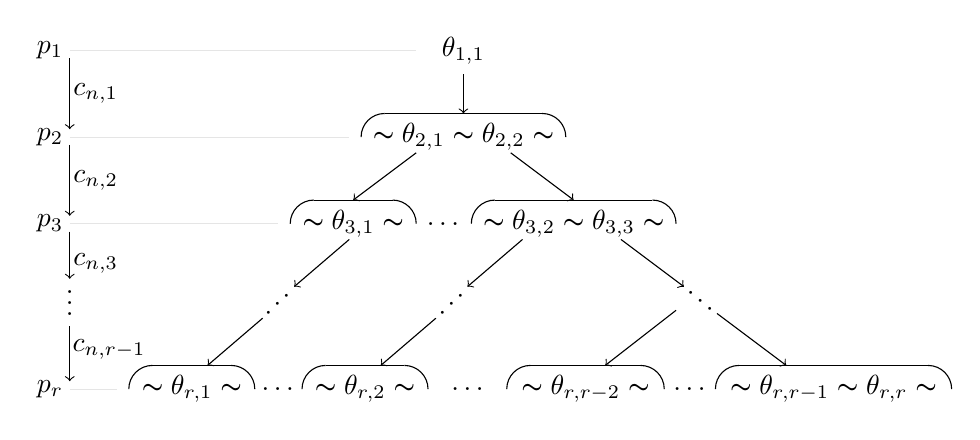
\begin{tikzpicture}
		\newcommand{\halfblob}[5]{ % #1: radius, #2: half-length, #3: x-coordinate, #4: y-coordinate, #5: name
			\draw (#3 - #2,#4 + #1) arc [start angle=90, end angle=180, radius=#1];
			\draw (#3 + #2 + #1,#4) arc [start angle=0, end angle=90, radius=#1];
			\draw (#3 - #2,#4 + #1) -- (#3 + #2,#4 + #1);
			%\draw (#3 - #2,#4 - #1) -- (#3 + #2,#4 - #1);
			\node at (#3,#4) {#5};
		}
		
		\node at (0,0) {$\theta_{1,1}$};
		\draw[->] (0,-0.3) -> (0,-0.8);
		\halfblob{0.3}{1}{0}{-1.1}{$\thicksim \theta_{2,1} \thicksim \theta_{2,2} \thicksim$}
		
		\draw[->] (-0.6,-1.3) -> (-1.4,-1.9);
		\halfblob{0.3}{0.5}{-1.4}{-2.2}{$\thicksim \theta_{3,1} \thicksim$}
		\draw[->] (0.6,-1.3) -> (1.4,-1.9);
		\halfblob{0.3}{1}{1.4}{-2.2}{$\thicksim \theta_{3,2} \thicksim \theta_{3,3} \thicksim$}
		\node at (-0.23,-2.2) {$\dots$};
		
		\draw[->] (-1.45,-2.4) -> (-2.15,-3);
		\node[rotate=43] at (-2.34,-3.2) {$\dots$};
		\draw[->] (-2.55,-3.4) -> (-3.25,-4);
		\halfblob{0.3}{0.5}{-3.45}{-4.3}{$\thicksim \theta_{r,1} \thicksim$}
		
		\draw[->] (0.75,-2.4) -> (0.05,-3);
		\node[rotate=43] at (-0.13,-3.2) {$\dots$};
		\draw[->] (-0.35,-3.4) -> (-1.05,-4);
		\halfblob{0.3}{0.5}{-1.25}{-4.3}{$\thicksim \theta_{r,2} \thicksim$}
		
		\draw[->] (2,-2.4) -> (2.8,-3);
		\node[rotate=-40] at (3.03,-3.2) {$\dots$};
		\draw[->] (2.7,-3.3) -> (1.8,-4);
		\halfblob{0.3}{0.7}{1.55}{-4.3}{$\thicksim \theta_{r,r-2} \thicksim$}
		\draw[->] (3.22,-3.34) -> (4.1,-4);
		\halfblob{0.3}{1.2}{4.7}{-4.3}{$\thicksim \theta_{r,r-1} \thicksim \theta_{r,r} \thicksim$}
		
		\node at (-2.33,-4.3) {$\dots$};
		\node at (0.08,-4.3) {$\dots$};
		\node at (2.9,-4.3) {$\dots$};
		
		%vertical arrows on the side
		\draw[->] (-5,-0.1) -> (-5,-1);
		\node at (-4.67,-0.55) {$c_{n,1}$};
		\draw[->] (-5,-1.2) -> (-5,-2.1);
		\node at (-4.67,-1.65) {$c_{n,2}$};
		\draw[->] (-5,-2.3) -> (-5,-2.9);
		\node at (-4.67,-2.7) {$c_{n,3}$};
		\node at (-5,-3.1) {$\vdots$};
		\draw[->] (-5,-3.5) -> (-5,-4.2);
		\node at (-4.5,-3.8) {$c_{n,r-1}$};
		
		%horizontal gray lines
		\draw[gray!20] (-5,0) -> (-0.6,0);
		\draw[gray!20] (-5,-1.1) -> (-1.45,-1.1);
		\draw[gray!20] (-5,-2.2) -> (-2.35,-2.2);
		\draw[gray!20] (-5,-4.3) -> (-4.4,-4.3);
		
		%look-ahead states
		\node at (-5.25,0) {$p_1$};
		\node at (-5.25,-1.1) {$p_2$};
		\node at (-5.25,-2.2) {$p_3$};
		\node at (-5.25,-4.3) {$p_r$};		
		
	\end{tikzpicture}
\end{center}
Note that, in this representation, we chose to represent 
$\theta_{i,i} \to_{c_i} w_{i} \, \theta_{i+1,i} \, w'_{i} \, \theta_{i+1,i+1} \, w''_i$ instead of 
$\theta_{i,i} \to_{c_i} w_{i} \, \theta_{i+1,i+1} \, w'_{i} \, \theta_{i+1,i} \, w''_i$ for all $i \in [r-1]$. 
But this distinction does not matter to the proof of the claim. 
%but because the order of nesting does not matter for nesting loops, 
%we can assume that branching is happening on the right without loss of generality (in fact 
%branching on the left makes the proof easier by excluding the case where $\bot$ occurs on the branching side). 
From now on we use $\thicksim$ to denote arbitrary sequences in $\QY^*$ which we will not use to find a nesting loop. 

\begin{proof}
We prove this by induction on $r$. 
Let $c$ be a $\Sigma$-context, $\theta$ a pair in $\QY$ and $w$ a sequence in $\QY^*$ with $\theta \to_{c} w$ and $|w| \geq B^{r+1}$. 
We split $c$ into atomic $\Sigma$-contexts $c'_1, \dots, c'_n$, then we have sequences $w_1, \dots, w_{n-1} \in \QY^*$ 
such that $\theta \to_{c'_1} w_1 \dots \to_{c'_{n-1}} w_{n-1} \to_{c'_n} w$. 
Let $i$ be the largest $i$ such that there is a pair $\theta'$ in sequence $w_i$ with $\theta' \to_{c'_{i+1} \cdots c'_n} w'$ and $|w'| \geq B^r$. 
If we had $|w'| \geq B^{r+1}$ then, because $c'_{i+1}$ is atomic, we would have a $\theta''$ in sequence $c'_{i+1}$ with $\theta'' \to_{c'_{i+2} \cdots c'_n} w''$ and $|w''| \geq B^r$. 
So $B^r \leq |w'| < B^{r+1} \leq |w|$. 
Therefore there is another pair $\theta_{2,1}$ in $w_i$ (other than $\theta'$) with $\theta_{2,1} \to_{c'_{i+1} \cdots c'_n} w''$ and $|w''| \geq 1$. 

Since $\theta' \to_{c'_{i+1} \cdots c'_n} w'$ and $|w'| \geq B^r$, we use the induction hypothesis on $theta'$ and $c'_{i+1} \cdots c'_n$. In order to prove the induction for $r+1$, we rename the $\Sigma$-contexts $c_1, \dots c_{r-1}$, look-ahead states $p_1, \dots, p_r$ and pairs $\theta_{i,j}$ (for $j \leq i \leq r$) into $\Sigma$-contexts $c_2, \dots c_{r}$, look-ahead states $p_2, \dots, p_{r+1}$ and pairs $\theta_{i+1,j+1}$ (for $j \leq i \leq r$). 
Then $c'_{i+1} \cdots c'_n = c_2 \cdots c_{r}$. 

Since $\theta_{2,1} \to_{c_2 \cdots c_r} w''$ with $|w''| \geq 1$, there are pairs $\theta_{3,1}, \dots, \theta_{n,1}$ such that $\theta_{n,1}$ appears in sequence $w''$ and, for all $i \in [r]$ with $i \geq 2$, $\theta_{i,1} \to_{c_i} w'_i \, \theta_{i+1,1} \, w''_i$ with $w'_i, w''_i \in \QY^*$. 
To conclude, we choose $c_1 = c'_1 \dots c'_i$, $p_1 = h(c_1)$ and $\theta_{1,1} = \theta$. 
\end{proof}

In order to find a nesting loop, we need two indexes $i$ and $j$ with: 
\begin{center}
	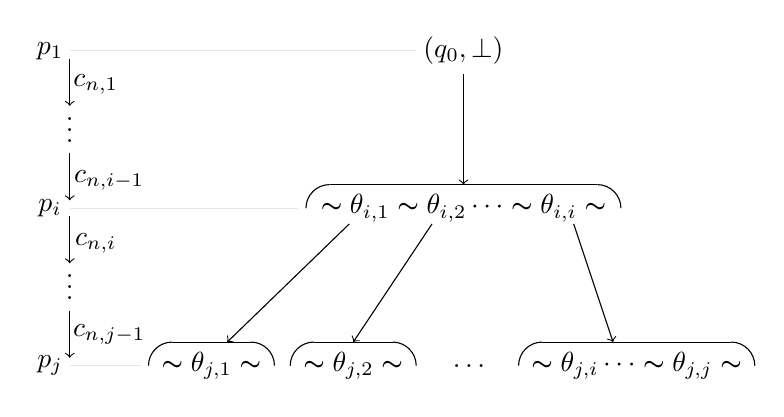
\begin{tikzpicture}
		\newcommand{\halfblob}[5]{ % #1: radius, #2: half-length, #3: x-coordinate, #4: y-coordinate, #5: name
			\draw (#3 - #2,#4 + #1) arc [start angle=90, end angle=180, radius=#1];
			\draw (#3 + #2 + #1,#4) arc [start angle=0, end angle=90, radius=#1];
			\draw (#3 - #2,#4 + #1) -- (#3 + #2,#4 + #1);
			%\draw (#3 - #2,#4 - #1) -- (#3 + #2,#4 - #1);
			\node at (#3,#4) {#5};
		}
		
		\node at (0,0) {$(q_0,\bot)$};
		\draw[->] (0,-0.3) -> (0,-1.7);
		\halfblob{0.3}{1.7}{0}{-2}{$\thicksim \theta_{i,1} \thicksim \theta_{i,2} \dots \thicksim \theta_{i,i} \thicksim$}
		
		\draw[->] (-1.45,-2.2) -> (-3,-3.7);
		\halfblob{0.3}{0.5}{-3.2}{-4}{$\thicksim \theta_{j,1} \thicksim$}
		
		\draw[->] (-0.4,-2.2) -> (-1.4,-3.7);
		\halfblob{0.3}{0.5}{-1.4}{-4}{$\thicksim \theta_{j,2} \thicksim$}
		
		\draw[->] (1.4,-2.2) -> (1.9,-3.7);
		\halfblob{0.3}{1.2}{2.2}{-4}{$\thicksim \theta_{j,i} \dots \thicksim \theta_{j,j} \thicksim$}
		\node at (0.1,-4) {$\dots$};
		
		%vertical arrows on the side
		\draw[->] (-5,-0.1) -> (-5,-0.7);
		\node at (-4.67,-0.43) {$c_{n,1}$};
		\node at (-5,-0.9) {$\vdots$};
		\draw[->] (-5,-1.3) -> (-5,-1.9);
		\node at (-4.5,-1.65) {$c_{n,i-1}$};

		\draw[->] (-5,-2.1) -> (-5,-2.7);
		\node at (-4.67,-2.45) {$c_{n,i}$};
		\node at (-5,-2.9) {$\vdots$};
		\draw[->] (-5,-3.3) -> (-5,-3.9);
		\node at (-4.5,-3.6) {$c_{n,j-1}$};
		
		%horizontal gray lines
		\draw[gray!20] (-5,0) -> (-0.6,0);
		\draw[gray!20] (-5,-2) -> (-2.1,-2);
		\draw[gray!20] (-5,-4) -> (-4.1,-4);
		
		%look-ahead states
		\node at (-5.25,0) {$p_1$};
		\node at (-5.25,-2) {$p_i$};
		\node at (-5.25,-4) {$p_j$};		
		
	\end{tikzpicture}
\end{center}
Formally, we require two indexes $i,j$ with $i < j < r$ which share the same:
\begin{itemize}
\item look-ahead state $h(c_{n,i}) = h(c_{n,j})$, 
\item pair $\theta_{i,i} = \theta_{j,j} \in \QY$, 
\item set of pairs $\{\theta_{i,\ell}\}_{0\leq \ell \leq i} = \{\theta_{j,\ell}\}_{0\leq \ell \leq j}$.  
\end{itemize}
We ensure the existence of such $i,j$ by taking $r \geq |P|\,|Q|\,(m+1) \, 2^{|Q| (m+1)} +1$ 
%(so $n = B^{|P|\,|Q|\,(m+1)\, 2^{|Q| (m+1)} +1}$) 
where $m$ is the maximum arity of states. 
%We ensure the existence of such $i,j$ by taking $r \geq |P|\,|\QY| \, 2^{|\QY|} +1$ 
%(so $n = B^{|P|\,|\QY|\, 2^{|\QY|} +1}$) with $|\QY| \leq |Q| \, (m+1)$ where $m$ is the maximum arity of states. 
We now show how to build the nesting loop from indexes $i,j$. 
We note $p = h(c_{n,i}) = h(c_{n,j})$, $(q_1,k_1) = \theta_{i,i} = \theta_{j,j}$ and 
$S = \{\theta_{i,\ell}\}_{0\leq \ell \leq i} = \{\theta_{j,\ell}\}_{0\leq \ell \leq j}$. 
We note $c' = c_{n,i}.c_{n,i+1}. \dots. c_{n,j-1}$. 
Note that $c'$ has a leaf labeled $p$ and $h(c')=p$. 
%drawing maybe

We need the sets $\{\theta_{i,\ell}\}_{0\leq \ell \leq i}$ and $\{\theta_{j,\ell}\}_{0\leq \ell \leq j}$ 
to be equal so that the pairs $\theta_{i,k}$ for $k \leq i$ loop on each other through the loop $c'$. 
Formally, noting $\theta'_0 = \theta_{j,i}$, for all $\theta'_k \in S$ for $k \in \N$, there exists 
$\theta'_{k+1} \in S$ such that $\theta'_k \to_c' \,\thicksim \theta'_{k+1} \thicksim$. 
Since $S \subseteq \QY$ is finite, there must be $n, m \in \N$ such that 
$\theta'_{n} = \theta'_{n+m}$ (with $m \geq 1$), so $\theta'_n \to_{c'^m} \,\thicksim \theta'_n \thicksim$. 
Also $(q_1,k_1) \to_{c'} \,\thicksim \theta'_0 \thicksim (q_1,k_1) \thicksim\,$ and $\theta'_0 \to_{c'^n} x_n$, 
so $(q_1,k_1) \to_{c'^{n+1}} \, \thicksim \theta'_n \thicksim (q_1,k_1) \thicksim\,$ and, for all $m' \in \N$: 
$(q_1,k_1) \to_{c'^{m'}} \, \thicksim (q_1,k_1) \thicksim \, \to_{c'^{n+1}} \, \thicksim \theta'_n \thicksim (q_1,k_1) \thicksim$. 
Finally, for $c = c'^{m(n+1)}$, we have 
$(q_1,k_1) \to_{c} \, \thicksim \theta'_n \thicksim (q_1,k_1)\thicksim$ and $\theta'_n \to_{c} \theta'_n$. 
So we have a \emph{nesting loop}. 

In conclusion, if $M$ is not finite nesting, then it is \emph{nested input pumpable}, and so it does not have linear size-to-height increase. 
\vspace{2mm}

The proof of Statement~(2) can be given in a very similar way as for~(1), here we only outline the changes to the notations which allow to adapt the proof of~(1) to~(2). 
We replace $\Sigma$-contexts with elements of the set $T_\Sigma(P)$ containing possibly several leafs labeled in $P$. The rest of the notational changes are consequences of this change. 
Given a $s \in T_\Sigma(P)$, we now consider the nesting of state calls called on distinct subtrees of $s$ with potentially distinct look-ahead states. We augment pairs in $\QY$ so as to include the look-ahead, so $\QY = \{ (q,k,p) \mid q \in Q^{(m)}, k \in [m] \cup \{\bot\}, p \in P\}$. The notation $(q,k,p) \to_s (q_1,k_1,p_1) \dots (q_n,k_n,p_n)$ means that $h(s)=p$ and calls to states $q_1, \dots, q_n$ on leafs of $s$ labeled $p_1, \dots, p_n$ resp.\ are nested on parameters $y_{k_1}, \dots, y_{k_n}$ along a path in $\widehat{M}_q(s)$. This means that, when concatenating contexts, we write $s(s_1, \dots, s_m)$ instead of $s\cdot s'$. 

For~(2), similarly to nesting loops for~(1), we define a \emph{yield nesting loop} as given by contexts $s_1, s_2 \in T_\Sigma(P)$, look-ahead states $p_1, p_2 \in P$ and triplets $(q_1,k_1,p_1), (q_2,k_2,p_2) \in \QY$ such that:
\begin{itemize}
\item $h(s_1) = p_1$, $h(s_2) = p_2$, $s_1$ has two leafs labeled $p_1$ and $p_2$, $s_2$ has one leaf labeled $p_2$, 
\item $\<q_1,p_1>$ is reachable, 
\item either $(q_1,k_1,p_1) \to_{s_1} \thicksim\, (q_2,k_2,p_2) \,\thicksim\, (q_1,k_1,p_1) \,\thicksim$ \\
\phantom{.} \hspace{2.5mm} or $(q_1,k_1,p_1) \to_{s_1} \thicksim\, (q_1,k_1,p_1) \,\thicksim\, (q_2,k_2,p_2) \,\thicksim$,
\item $(q_2,k_2,p_2) \to_{s_2} \thicksim\, (q_2,k_2,p_2) \,\thicksim$. 
\end{itemize}
  
We say that $M$ is \emph{yield nested input pumpable} when it has either a \emph{yield nesting loop} or a \emph{nesting loop}. 
Note that the existence of either of these loops falsifies the linear height increase property. 
To prove~(2) we prove that infinite yield nesting implies the existence of either a yield nesting loop or a nesting loop. That proof works similarly to~(1): $M$ is not fynest so we can find large enough nesting sequences (but with the new definition of $\to_s$), find a repeating triplet $(q_1,k_1,p_1)$, pump the loop enough times that a triplet $(q_2,k_2,p_2)$ loops onto itself. Note that if the nested calls to $(q_1,k_1,p_1)$ and $(q_2,k_2,p_2)$ in $(q_1,k_1,p_1) \to_{s_1} \,\thicksim (q_2,k_2,p_2) \thicksim (q_1,k_1,p_1) \thicksim$ are on the same leaf in $s_1$ (with $p_1 = p_2$), then we get a nesting loop (otherwise we get a yield nesting loop). 



%%old version of definition of \to_s
%(Old version.) When considering the nesting of states, we want to specify the look-ahead the state is called upon, and in which parameter the nesting occurs. We define the set $\QY = \{ (q,p,y_k) \mid q \in Q^{(m)}, p \in P, y_k \in Y_m \cup \{\bot\}\}$ of nesting state configurations. We use configuration $(q,p,\bot)$ to denote the state called at the bottom of a nesting chain, with no state calls in any of its parameters. 
%
%For a $\Sigma$-context $s$ containing a leaf $p$, we write $(q,h(s),\bot) \to_s (q_1,p,y_{k_1}) \dots (q_{n-1},p, y_{k_{n-1}}) (q_n,p,\bot)$ when state calls $\<q_1,p>, \<q_2,p>, \dots$ appear nested in $M_{q}(s)$, with $\<q_2,p>$ appearing in parameter $y_{k_1}$ of $\<q_1,p>$, $\<q_3,p>$ appearing in parameter $y_{k_2}$ of $\<q_2,p>$ and so on. We write $(q,h(s),y_k) \to_s (q_1,p,y_{k_1}) \dots (q_n,p,y_{k_n})$ when $(q,h(s),\bot) \to_s (q_1,p,y_{k_1}) \dots (q_{n-1},p, y_{k_{n-1}}) (q_n,\bot)$ and parameter $y_k$ of $q$ appears in parameter $y_{k_n}$ of $\<q_n,p>$. 
%%For a $\Sigma$-context $s$ containing look-ahead state $p$, we write $(q_0,p_0,y_{k_0}) \to_s (q_1,p,y_{k_1}) \dots (q_n,p,y_{k_n})$ when $p_0 = h(s)$ and, in $M_{q_0}(s)$, state calls $\<q_1,p>, \<q_2,p>, \dots$ appear nested on parameters $y_{k_1}, y_{k_2}, \dots$, along a path leading to parameter $y$. 
%%We write $(q_0,p_0,\bot) \to_s (q_1,p,x_1) \dots (q_n,p,x_n)$ when $p_0 = h(s)$ and there exists exactly one $x_i$ with $x_i = \bot$ such that, in $M_{q_0}(s)$, state calls $\<q_1,p>, \dots$ appear nested on parameters $y_{k_1}, y_{k_2}, \dots$, along a path leading to parameter $y$. 
%Note that $\to_s$ is closed under subsequence on the right (i.e.\ we can "forget" part of the nested configurations). 
%We extend the relation $\to_s$ so that it is commutative and compatible with concatenation of sequences in $\QY^*$, i.e.\ so that $w \to_s w_2 w_1$ when $w \to_s w_1 w_2$, and $w_1 w_2 \to_s w'_1 w'_2$ when both $w_1 \to_s w'_1$ and $w_2 \to_s w'_2$, for all $w, w_1, w'_1, w_2, w'_2 \in \QY^*$. 
%Given two $\Sigma$-contexts $s$ and $s'$ containing look-ahead states $p$ and $p'$, if $p = h(s')$, then $s\cdot s'$ denotes the $\Sigma$-context obtained from $s$ by replacing $p$ with $s'$. Note that, for all $a \in \QY$ and $w \in \QY^*$, $a \to_{s\cdot s'} w$ if and only if there exists $w' \in \QY^*$ such that $a \to_s w'$ and $w' \to_{s'} w$. 
%%We sometimes write $\to$ instead of $\to_s$ when $s$ is obvious from context or does not matter. 
%
%
%%definition of nesting loops
%(Definition of nesting loops.) We can now define \emph{nesting loops}, whose existence characterizes \emph{nested input pumpability}. 
%A \emph{nesting loop} is given by a $\Sigma$-context $s$ and two configurations $(q_1,p,y_i)$ and $(q_2,p,y_j) \in \QY$ such that: $\<q_1,p>$ is reachable, $(q_1,p,y_i) \to_s (q_2,p,y_j) (q_1,p,y_i)$ and $(q_2,p,y_j) \to_s (q_2,p,y_j)$. Note that $y_i$ could be either $\bot$ or a parameter of $q_1$ (these two cases represent the two cases in point 2. of the definition of nested input pumpability), but in either case $y_j \neq \bot$. 
%
%
%%\begin{claim}
%%If $M$ has a nesting loop then $M$ is not of linear size-to-height increase. 
%%\end{claim}
%%
%%\begin{proof}
%%We prove this by pumping the loop: pumping $n$ times gives either $(q_1,y_i) \to_{s^n} (q_1,y_i) (q_2,y_j)^n$ or $(q_1,y_i) \to_{s^n} (q_2,y_j)^n (q_1,y_i)$. Since $\<q_1,p>$ is reachable, there exists a $\Sigma$-context $s_0$ which leads to the state call $\<q_1,p>$. For all input tree $t \in L_p$, the output of $M$ on input $s_0(s^n(t))$ nests $n$ calls to state $q_2$ on tree $t$ (nested along parameter $y_j$). The input size is $|s_0| + n.|s| + |t|$ and the output height is at least $n.d$ where $d$ is the maximum depth of parameter $y_j$ in $q_2(t)$. 
%%If $M$ was of linear size-to-height increase we would have a bound $B$ such that $B.(|s_0| + n.|s| + |t|)\geq n.d$ for all $n$, so $B.|s| \geq d$. 
%%Since $M$ is depth proper, there is no upper bound for the depth $d$ where $y_j$ occurs in $q_2(t)$ for $t \in L_p$, so $M$ can not be of linear size-to-height increase. 
%%\end{proof}
%
%We now only need to prove that if $M$ is not finite nesting then it has a nesting loop. We assume that $M$ is not finite nesting, so for all $n \in \N$ there exists a $Sigma$-context $s$ and a configuration sequence $w \in \QY^n$ such that $(q_0,h(s),\bot) \to_s w$. We decompose $\Sigma$-context $s$ into a concatenation $s_1\cdot s_2\cdot \dots \cdot s_k$ of atomic $\Sigma$-contexts (i.e.\ context whose hole is at depth $1$) and we get: 
%$(q_0,h(s),\bot) \to_{s_1} x_{1,1} \dots x_{1,m_1} \to_{s_2} \dots \to_{s_m} x_{k,1} \dots x_{k,m_k}$ with $x_{i,j} \in \QY$ for all $i,j$ and $m_k = n$. 
%We can represent this structure of nested state calls as a \emph{configuration tree}:
%%tikz picture: configuration tree: $(q_0,h(s),\bot) \to_{s_1} x_{1,1} \dots x_{1,m_1} \to_{s_2} \dots \to_{s_m} x_{k,1} \dots x_{k,m_k}$
%%% Figure environment removed
%
%We say that a configuration tree is a $k$-comb if it is of the form:
%%tikz picture: $k$-comb
%\begin{center}
%\begin{tikzpicture}
%\node {$(q_0,p_0,\bot)$} [sibling distance = 12mm, level distance = 9mm]
%child {node {$x_{1,1}$}
%	child {node {$x_{2,1}$}
%		child {node {$x_{3,1}$}
%			child {node[rotate=57] {$\dots$}
%				child {node {$x_{k,1}$}
%				}
%				child[missing]
%			}
%			child[missing]
%		}
%		child[missing]
%	}
%	child {node {$x_{2,2}$}
%		child {node {$x_{3,2}$}
%			child {node[rotate=57] {$\dots$}
%				child {node {$x_{k,2}$}
%				}
%				child[missing]
%			}
%			child[missing]
%		}
%		child {node {$x_{3,3}$}
%			child {node[rotate=57] {$\dots$}
%			}
%			child {node[rotate=-57] {$\dots$}
%				child {node {$x_{k,k-1}$}
%				}
%				child {node {$x_{k,k}$}
%				}
%			}
%		}
%	}
%}
%;
%\node at (0,-4.5) {$\dots$};
%
%%other version:
%%\node {$(q_0,p_0,\bot)$} [sibling distance = 12mm, level distance = 10mm]
%%child {node {$x_{1,1}$}
%%	child {node {$x_{2,1}$}
%%		child {node[rotate=58] {$\dots$}
%%			child {node {$x_{k-1,1}$}
%%				child {node {$x_{k,1}$}
%%				}
%%				child[missing]
%%			}
%%			child[missing]
%%		}
%%		child[missing]
%%	}
%%	child {node {$x_{2,2}$}
%%		child {node[rotate=58] {$\dots$}
%%			child {node {$x_{k-1,2}$}
%%				child {node {$x_{k,2}$}
%%				}
%%				child[missing]
%%			}
%%			child[missing]
%%		}
%%		child {node[rotate=-58] {$\dots$}
%%			child[missing]
%%			child {node {$x_{k-1,k-1}$}
%%				child {node {$x_{k,k-1}$}
%%				}
%%				child {node {$x_{k,k}$}
%%				}
%%			}
%%		}
%%	}
%%}
%%;
%%\node at (0,-5) {$\dots$};
%\end{tikzpicture}
%\end{center}
%\vspace{-2mm}
%
%In configuration trees obtained by decomposing a $\Sigma$-context into atomic contexts, nodes have their arity bound by the nesting on the right-hand-side of rules of $M$. Noting this bound $B$, and for all $k \in \N$, any configuration tree with $B^{k+1}$ leafs and obtained by atomic decomposition can be pruned into a $k$-comb. 
%
%Formally, we prove this by induction on $k$. The allowed pruning operations are: $(a)$ remove a node and all its descendants, $(b)$ remove all nodes at a given depth by merging them with their parent node. Note that the nesting statements represented by the trees remain true when pruned. Also, pruned trees preserve the property: for all depth $i<k$, noting $x_{i,1}, \dots, x_{i,m_i}$ the nodes at depth $i$ and $x_{i+1,1}, \dots, x_{i+1,m_{i+1}}$ the nodes at depth $i+1$, there is a $\Sigma$-context $s_i$ such that:
%\vspace{-2mm}
%
%\[x_{i,1} \dots x_{i,m_i} \to_{s_i} x_{i+1,1} \dots x_{i+1,m_{i+1}}\]
%\vspace{-3mm}
%
%We now argue that by taking a big enough $k$-comb we ensure the existence of a nesting loop. We take $k= |\QY|.2^{|\QY|} +1$. Such a $k$-comb must have two depths $i,j$ with $i<j\leq k$ which share the same: 
%\begin{enumerate}
%\item configuration $(q_1,p,y_i) = x_{i,i} = x_{j,j}$ (the configuration on the spine of the comb, i.e.\ the right-most node at depth $i$ and $j$), 
%\item set of configurations $S= \{x_{i,\ell}\}_{0\leq \ell \leq i} = \{x_{j,\ell}\}_{0\leq \ell \leq j}$ (the sets of all configurations appearing at depth $i$ and $j$). 
%\end{enumerate}
%%Note that $k= |\QY|.2^{|\QY|/ |P|} +1$, where $|P|$ is the number of look-ahead states, would be enough because nodes of a same depth have the same $p$, but when adapting this proof to point~(2) we would need $k= |\QY|.2^{|\QY|} +1$. 
%So we have a $\Sigma$-context $s$ such that $(q_1,p,y_i) \to_s w_3 (q_1,p,y_i)$ and $w_1 \to_s w_2$ with $w_1, w_2, w_3 \in S^*$ and all configuration $x \in S \setminus \{(q_1,p,y_i)\}$ appears at least once in $w_1$ and once in $w_2 w_3$: 
%% tikzpicture of the loop s
%\begin{center}
%\begin{tikzpicture}
%\node at (-2,0) {$\phantom{B}$} [sibling distance = 12mm, level distance = 9mm]
%child {node[rotate=55] {$\dots$}
%	child {node {$\phantom{B}$}}
%	child[missing]
%}
%child[missing]
%;
%
%\node {$\phantom{B}$} [sibling distance = 12mm, level distance = 9mm]
%child {node[rotate=55] {$\dots$}
%	child {node {$\phantom{B}$}}
%	child[missing]
%}
%child[missing]
%;
%
%\node at (1,0) {$(q_1,p,y_i)$} [sibling distance = 12mm, level distance = 9mm]
%child {node[rotate=55] {$\dots$}
%	child {node {$\phantom{B}$}}
%	child[missing]
%}
%child {node[rotate=-55] {$\dots$}
%	child {node {$\phantom{B}$}}
%	child {node {$(q_1,p,y_i)$}}
%}
%;
%
%\newcommand{\blobby}[5]{ % #1: radius, #2: x1-coordinate, #3: x2-coordinate, #4: y-coordinate, #5: name
%	\draw (#2,#4 + #1) arc [start angle=90, end angle=270, radius=#1];
%	\draw (#3,#4 - #1) arc [start angle=-90, end angle=90, radius=#1];
%	\draw (#2,#4 + #1) -- (#3,#4 + #1);
%	\draw (#2,#4 - #1) -- (#3,#4 - #1);
%	\node at ($(#2,#4)!0.5!(#3,#4)$) {#5};
%}
%
%\blobby{0.23}{-2}{0}{0}{$w_1$}
%\blobby{0.23}{-3.2}{-1.2}{-1.8}{$w_2$}
%\blobby{0.23}{-0.2}{1}{-1.8}{$w_3$}
%
%\node at (-1.55,-0.9) {$\dots$};
%\end{tikzpicture}
%\end{center}
%
%Let $x_0 \in S$ be a configuration in $w_3$ (we can do so because $|w_3| = j-i \geq 1$). 
%Because $w_1 \to_s w_2$, we know that each configuration $x_k \in S$ has a $x_{k+1} \in S$ such that $x_k \to_s x_{k+1}$. Because $S \subseteq \QY$ is finite, there must be $n, m \in \N$ such that $x_{n} = x_{n+m}$ (with $m \geq 1$), so $x_n \to_{s^m} x_n$. Also $(q_1,p,y_i) \to_s (q_1,p,y_i)\, x_0$ and $x_0 \to_{s^n} x_n$, so $(q_1,p,y_i) \to_{s^{n+1}} (q_1,p,y_i)\, x_n$ and, for all $m' \in \N$: $(q_1,p,y_i) \to_{s^{m'}} (q_1,p,y_i) \to_{s^{n+1}} (q_1,p,y_i)\, x_n$. Finally, for $s_\ell = s^{m(n+1)}$, we have $(q_1,p,y_i) \to_{s_\ell} (q_1,p,y_i)\, x_n$ and $x_n \to_{s_\ell} x_n$. So we have a \emph{nesting loop}. 
%
%In conclusion, if $M$ is not finite nesting, then it is \emph{nested input pumpable}, and so it does not have linear size-to-height increase. 
%\vspace{2mm}

%The proof of Statement~(2) can be given in a very similar way as for~(1), here we only outline the changes to the notations which allow to adapt the proof of~(1) to~(2). 
%First we replace $\Sigma$-contexts with regular contexts (i.e.\ elements of the set $T_\Sigma(P)$) containing possibly several leafs in $P$. The rest of the notational changes are consequences of this change. 
%For $s \in T_\Sigma(P)$, the notation $(q,p,y) \to_s (q_1,p_1,y_{k_1}) \dots (q_n,p_n,y_{k_n})$ means that calls to states $q_1, \dots, q_n$ are nested along a path in $M_q(s)$, but now these calls can be on different leafs of $s$. This means that, when concatenating contexts, we use $s(s_1, \dots, s_m)$ instead of $s\cdot s'$. 
%
%For~(2), similarly to nesting loops for~(1), we define a \emph{yield nesting loop} as given by a pair of contexts $s_1, s_2 \in T_\Sigma(P)$, and configurations $(q_1,p_1,y_i), (q_2,p_2,y_j) \in \QY$ such that: $\<q_1,p_1>$ is reachable, $(q_1,p_1,y_i) \to_{s_1} (q_2,p_2,y_j) (q_1,p_1,y_i)$, and $(q_2,p_2,y_j) \to_{s_2} (q_2,p_2,y_j)$. 
%We say that $M$ is \emph{yield nested input pumpable} when it has either a \emph{yield nesting loop} or a \emph{nesting loop}. 
%Note that the existence of either of these loops falsifies the linear height increase property. 
%To prove~(2) we prove that infinite yield nesting implies the existence of either a yield nesting loop or a nesting loop. That proof works similarly to~(1): existence of $k$-combs for any $k$ (but with the new definition of $\to_s$), find a repeating configuration $(q_1,p_1,y_i)$ on the spine of the comb, pump the loop enough times that a configuration $(q_2,p_2,y_j)$ comes onto itself. Note that if the nested calls to $(q_1,p_1,y_i)$ and $(q_2,p_2,y_j)$ in $(q_1,p_1,y_i) \to_{s_1} (q_2,p_2,y_j)\, (q_1,p_1,y_i)$ are on the same leaf in $s_1$, then we get a nesting loop (otherwise we get a yield nesting loop). 

%
%%Paul's version
%Because $M$ is depth-proper, for each $q \in Q^{(m)}, i \in [m], p \in P$ and 
%$n \in \N$, there is $t \in L_p$ such that $\he{\lcop{M_q(t)}_{\{y_i\}}} > n$. 
%We can ensure the existence of a productive loop in $t$ by taking 
%$n = 1+ \text{mhr} . k^{|Q| . |P|}$ where $k$ is the maximum arity of input trees. 
%Noting $t_j$ the tree where the loop is pumped $j$ times, we get 
%\[\he{\lcop{M_q(t_j)}_{\{y_i\}}} > c_s.|t_j| ~~~~\text{ and }~~~~ 
%\he{\lcop{M_q(t_j)}_{\{y_i\}}} > c_h.\he{t_j}\] 
%for all $j \geq 1$, 
%where $c_s$ and $c_h$ are strictly positive constants that depend on $M, q, i$ and $p$. 
%We can make $c_s$ and $c_h$ only dependent on $M$ by taking their maximum over 
%the possible $q \in Q^{(m)}, i\in [m]$ and $p \in P$. 
%
%To prove~(1), assume that $M$ is not fnest.
%We will show that this implies that $M$ does not have LSHI.
%For all $n \in \N$, there is $s \in T_\Sigma(P)$ with one occurrence of $P$ 
%such that there are at least $n$ nested occurrences of $P$ in $\he{\hat{M}(s)}$. 
%By taking $n$ big enough, we can get any number of nested calls of 
%\emph{the same state} $q$, nested in \emph{the same parameter} $y_i$ of $q$. 
%For all $n \in \N$, we note $s_{n} \in T_\Sigma(P)$ the tree with one occurrence of $P$ 
%such that there are at least $n$ occurrences of 
%$\langle q,p \rangle$ nested along parameter $y_i$ in $\he{\hat{M}(s)}$, 
%for some $q \in Q^{(m)}, i \in [m]$ and $p \in P$. We note $u_n$ such that $s_n/u_n \in P$, 
%and $t_{n,j} = s_n[u_n \leftarrow t_j]$ for all $n,j \in \N$. 
%For each $n$, there is $j_n$ such that $|t_{j_n}| > |s_n|$, so $|t_{j_n}| > |t_{n,j_n}|/2$. 
%Then, for all $n \in \N$:
%\[\he{M(t_{n,j_n})} \geq n.\he{\lcop{M_q(t_{j_n})}_{\{y_i\}}} > n.c_s.|t_{j_n}| > n.c_s.|t_{n,j_n}|/2 \]
%If $M$ had LSHI then there would be a constant $c$ such that \\
%$c > \he{M(t_{n,j_n})}/|t_{n,j_n}| > n.c_s/2$ for all $n \in \N$. 
%This is a contradiction, so $M$ does not have LSHI. 
%
%To prove~(2), assume that $M$ is not fynest.
%We will show that this implies that $M$ does not have LHI.
%For all $n \in \N$, there is $s \in T_\Sigma(P)$ 
%such that there are at least $n$ nested occurrences of $P$ in $\he{\hat{M}(s)}$. 
%By taking $n$ big enough, we can get any number of nested calls of 
%\emph{the same state} $q$, nested in \emph{the same parameter} $y_i$ of $q$, 
%applied to \emph{the same look-ahead state} $p$. 
%For all $n \in \N$, we note $s_{n} \in T_\Sigma(P)$ the tree 
%such that there are at least $n$ occurrences of 
%$\langle q,p \rangle$ nested along parameter $y_i$ in $\he{\hat{M}(s)}$, 
%for some $q \in Q^{(m)}, i \in [m]$ and $p \in P$. 
%We note $t_{n,j} = s_n[p \leftarrow t_j]$ for all $n,j \in \N$. 
%For each $n$, there is $j_n$ such that $\he{t_{j_n}} > \he{s_n}$, so $\he{t_{j_n}} > \he{t_{n,j_n}}/2$. 
%Then, for all $n \in \N$:
%\[\he{M(t_{n,j_n})} \geq n.\he{\lcop{M_q(t_{j_n})}_{\{y_i\}}} > n.c_h.\he{t_{j_n}} > n.c_h.\he{t_{n,j_n}}/2 \]
%If $M$ had LHI then there would be a constant $c$ such that \\
%$c > \he{M(t_{n,j_n})}/\he{t_{n,j_n}} > n.c_h/2$, for all $n \in \N$.
%This is a contradiction, so $M$ does not have LHI. 
%
%\qed
\end{proof}

From Theorem~\ref{th:proper} and Lemmas~\ref{lm:decidable},~\ref{lm:easy}, and~\ref{lm:nest} we obtain
our following main theorem.

\begin{theorem}
Let $M$ be an mttr. 
Then 
(1)~it is decidable whether or not $M$ has linear size-to-height increase
(2)~it is decidable whether or not $M$ is linear height-increase.
\end{theorem}

\section{Conclusions}

We have proven that for a given macro tree transducer (with look-ahead) it
is decidable whether or not it has linear height increase (LHI) and,
whether or not it has linear size-to-height increase (LSHI).
Both decision procedures rely on a novel normal form that is called
``depth-proper'' normal form. Roughly speaking the normal form requires
that each parameter of every state of the transducer appears at
arbitrary large depths in output trees generated by that state (and for a given
look-ahead state). 

One major open problem in the field is to prove a Conjecture of Joost Engelfriet
(from around the year 2000), that the translation of an mttr can be defined by
an attributed tree transducer (atts) if and only if the translation 
has ``linear size to number of distinct output subtrees'' increase.
Note that deciding such property is out of reach (it is at least as difficult as deciding
equivalence of atts). To prove this characterization, different loops need to
be considered which produce unbounded numbers of states in (partial) output trees.
We believe that the depth normal form will be instrumental in reducing the number of
different such loops that must be considered and therefore will be of great help
in proving the conjecture.

\iffalse
Our construction
of the normal form removes parameters that only appear at bounded depth. 
Once in depth-normal form, we can reduce the check for LHI and LSHI
to the finiteness of ranges of mtts.

Both LHI and LSHI are natural properties and have several useful applications.
For instance, if an mtt does not have LHI, then we know that it cannot be realized
by a top-down or a bottom-up tree transducer. And, if an mtt does not have LSHI, then
we know that it cannot be realized by any attributed tree transducers.
%
%The most prevailing open problem is to solve the conjecture (see Introduction) that
%the translation of an mtt can be realized by an attributed tree transducer if and only
%if the translation is of LSOI (linear size-to-number-of-distinct-output-subtrees).
%In this paper we merely show that \emph{deciding} if an mtt is of LSOI is as
%hard as deciding equivalence of attributed transducers (a long standing difficult open problem).
%We believe that the depth-proper normal form will be helpful in solving the conjecture.
%Intuitively, loops need to be considered only if they produce an arbitrary number of copies of
%states with parameters. In these loops we can exclude certain state nestings, due to
%the normal form.
%
An interesting open problem is the question whether or not the mtt hierarchy
(generated by sequential compositions of mtts) collapses for LSHI or for LHI.
By this we mean (in the case of LSHI), whether or not there exists some number $n$ such that
$
\cup \{ \text{MTT}^k \mid k\geq 1 \} \cap \text{LSHI} \subseteq \text{MTT}^n.
$
Note that for linear size increase, the hierarchy collapses~\cite{DBLP:journals/acta/EngelfrietIM21}
to level one, i.e., $n=1$.
It can be shown by an easy counting argument (similar as when proving that sequential composition
of mttrs gives rise to a hierarchy that is strict at each level) that no such $n$ exists:
consider compositions of the translation $\tau$ that takes a binary
tree $s$ as input and outputs a full binary tree of height $|s|$.
Then $\tau_k\in
\text{MTT}\cap\text{LSHI})^{k+1} - \text{MTT}\cap\text{LSHI})^k$.
Thus, the MTT hierarchy restricted to linear size-to-height increase remains to
be strict at each level.

The corresponding question for LHI is open, i.e., we do not know whether or not
the MTT hieararchy restricted to linear height increase is strict.
We do have a candidate translation that would show (for level two) both, that a two-fold composition of
mtts of LHI can do strictly more than a single mtt, and, that two-fold compositions
that are of LHI are strictly more than a single mtt:
input trees are monadic trees of the form $a^n(e)$ and output trees are full binary
trees of height $n$, at the leaves of which are monadic trees that represent
the Dewey paths of those ``leaves'' of the binary tree.
E.g.
$a(a(e))$ is translated to
$
f(f(1(1(e)), 1(2(e))), f(2(1(e)), 2(2(e)))).
$
Note that if we output \emph{reverse} such Dewey paths, then the translation
indeed can be realized by a single mtt (see, e.g., Fig.~6.2 in~\cite{DBLP:series/eatcs/FulopV98}).
Thus, the second transducer of the composition reverses the reverse Dewey paths.
\fi

%
% Figure environment removed


\section{Computational Complexity}
\label{sec:complexity}
In this section, we provide a comparison of the computational complexity according to the attention operations used in the existing approaches. We first define variables that define the number of elements. $N$, $M$, and $T$ correspond to the number of agents, lane elements, and time steps, respectively. $T$ can be decomposed into two variables, $T_p$ and $T_f$, which refer to past and future time steps, respectively. In general, the number of agents dominates the computation, then, the number of lanes followed by the fixed number of time steps, \eg $T=50$~($N>M>T$). While the number of lanes $M$ stays mostly uniform across scenes, the number of agents $N$ might vary significantly even for the same scene.

As addressed in the SceneTransformer~\cite{Ngiam2022ICLR}, directly applying attention to both time and agent axes results in high overhead, with the computational complexity of $\mathcal{O}((NT + M)^2)$ where $N$ is the number of agents, $M$ is the number of lane segments and $T$ is the number of time steps including both past and future. SceneTransformer reduces it to $\mathcal{O}(NT^2 + N^2T + NTM)$ with factorized attention over time and agent axes. 

Autobot~\cite{Girgis2022ICLR} does not include lane elements in their factorized attention steps. Contrary to SceneTransformer, their encoding and decoding phases consider only past and future time steps, respectively, resulting in the complexity of $\mathcal{O}(N{T_p}^2 + N^2{T_p} + N{T_f}^2 + N^2{T_f})$ where $T_p$ denotes the number of past time steps and $T_f$ denotes the number of future time steps.

HiVT~\cite{Zhou2022CVPR} does not use the standard multi-axis factorized attention but embraces a more efficient type of temporal interaction by considering only one agent for each time step and attending to only one feature over different time steps. Since HiVT follows an agent-centric approach and calculates agent features independently from each other, considering only one agent in their local scene does not result in information loss. However, the agent-centric approach comes with the overhead of $N$ runs of the same procedure. Considering scene normalization for each agent and global interaction in the end, HiVT has the overall complexity of
$\mathcal{O}(N^2{T_p} + N{T_p}^2 + NM)$. 

ADAPT has a clear advantage in terms of computational complexity over the existing approaches. Our computation is not bounded by $T$ as our subgraphs in vectorized encoder handle the temporal reasoning. Since we calculate the attention over only agents and lanes, ADAPT has the complexity of $\mathcal{O}(N^2 + NM + M^2)$ resulting from the attention operations in the interaction modeling. Removing the number of time steps $T$ out of the equation is the main reason behind the efficiency gain of ADAPT.



\bigskip

%\subsection*{Acknowledgements}
\textbf{Acknowledgements.}\quad
We thank the anonymous reviewers of a previous version of this paper
for their very careful and critical comments which hugely helped to improve the paper.

\newpage

%CASE: COMPOSITION OF TOTAL TRANSDUCERS\\
%better time complexity as modification of $T_1$ and look-ahead are not necessary.\\
%Construction of  $M$, $O(T_1^{T_2})$

\bibliographystyle{splncs04}% the mandatory bibstyle
\bibliography{mybib}

\newpage
\appendix
%!TEX root = ICALP_main.tex
\section*{Appendix}

\subsection*{Proof of Lemma~\ref{lm:nd}}

Statement of the lemma:
Let $\Delta$ be a ranked alphabet, $m\geq 1$, $Z\subseteq Y_m$, and
$t\in T_\Delta(Y_m)$.
(1)~$t=\lcop{t}_Z[u\leftarrow t/u\mid u\in\mathcal{U}(\lcop{t}_Z)]$.
(2)~$\paras{\lcop{t}_Z} = \paras{t}$. 

\smallskip

\begin{proof}
The proof is by induction on the structure of $\lcop{t}_Z$.
Let us denote the substitution $[u\leftarrow t/u\mid u\in\mathcal{U}(\lcop{t}_Z)]$
by $[t]$.
%
There are three cases.

Case 1: $t = y\in Z$. Then $\mathcal{U}(\lcop{t}_Z)=\emptyset$.
Hence $\lcop{t}_Z[t]=\lcop{y}_Z$. The latter equals $y=t$ by 
the definition of $\lcop{.}_Z$. Thus~(1)~holds. Also 
$\paras{\lcop{t}_Z}=\{y\}=\paras{t}$ and so~(2)~holds. 
%the definition of $\lcop{.}_Z$. Thus~(1)~holds and~(2)~holds for $u=\epsilon$.

Case 2: $\paras{t} \cap Z = \emptyset$. Then $\lcop{t}_Z = \paras{t} = Z' \subseteq Y_m$ 
by the definition of $\lcop{.}_Z$, and $\mathcal{U}(\lcop{t}_Z)=\{ \epsilon \}$. Hence
$\lcop{t}_Z[t] = \lcop{t}_Z[\epsilon\leftarrow t/\epsilon = t] = t$ which proves~(1). 
Again~(2)~holds 
because $\paras{\lcop{t}_Z}=\paras{\paras{t}}=\paras{t}$. 
%for $u=\varepsilon$ for each $y \in \paras{t}$ i.e.\ $y$ occurring in $t$.

Case 3: \(\paras{t}\cap Z\ne\emptyset\). Then $t=\delta(t_1,\dots,t_n)$, 
$\delta\in\Delta^{(n)}$, $n\geq 0$,
and $t_1,\dots, t_n\in T_\Delta(Y_m)$.
To show~(1) we obtain from the definition of $\lcop{t}_Z$ that
\[
\lcop{t}_Z[t]=\delta(\lcop{t_1}_Z,\dots,\lcop{t_n}_Z)[t]
= \delta(\lcop{t_1}_Z[t_1],\dots,\lcop{t_n}_Z[t_n]),
\]
where for $i\in[n]$, $[t_i]$ denotes the substitution
$[u\leftarrow t_i/u\mid u\in\mathcal{U}(\lcop{t_i}_Z)]$.
By induction the latter equals $\delta(t_1,\dots,t_n)=t$.
Finally~(2)~is implied by the induction hypothesis:
$\paras{\lcop{t}_Z}=\bigcup_{j\in[n]} \paras{\lcop{t_j}_Z}
=\bigcup_{j\in[n]} \paras{t_j}= \paras{t}$
%To show~(2), assume $y\in Y_m$ occurs in $t$.
%Thus, $n\geq 1$ and there exists an $i\in[n]$
%such that $y$ occurs in $t_i$.
%By induction of Statement~(2), there exists a leaf $u$ of $t_i$ such that 
%Statement~(2) holds (for $u$ and $t_i$); therefore Statement~(2) holds
%for $iu$ and $t$.
%\qed
\end{proof}

\subsection*{Proof of Lemma~\ref{lm:lcop_finite}}

Statement of the lemma:
Let $M$ be an mtt, $q$ a state of $M$, and $p$ a look-ahead state of $M$
such that $Y(q,p)\not=\emptyset$.
Then $\lcop{M_q(L_p)}_{Y(q,p)}$ is finite.

\smallskip

\begin{proof}
Assume that $Y_{q,p}=\{y_{j_1},\dots,y_{j_n}\}$ where $n\geq 1$.
It follows from the definition of $Y(q,p)$ that for each $i\in[n]$ there exists
a number $d_i$ such that $y_{j_i}$ occurs at depth $\leq d_i$ in 
any tree in $M_q(L_p)$. Let $d$ be the maximum of all numbers in
$\{ d_1,\dots,d_n\}$. Then every parameter in $Y(q,p)$ occurs at depth $\leq d$ in
any tree in $M_q(L_p)$. It follows from the definition of $U=\lcop{M_q(L_p)}_{Y(q,p)}$
that every node of a tree in $U$ has depth $\leq d$. Thus, $U$ is finite.
%\qed
\end{proof}


\subsection*{Example of Constructing a Depth Proper MTTR}

%\newcommand\qid{q_{\mathrm{id}}}
Let \(M=(\{q_0,q_1,q_2,q_3,q_4,\qid\},\{p\},\Sigma,$ $\Delta,q_0,R,h_0)\)
with \(\Sigma=\{a^{(1)},e^{(0)}\}\) and 
%\(\Delta=\{a_1^{(1)},a_2^{(2)},a_3^{(2)},a_4^{(1)},f^{(2)},g^{(3)},e^{(0)}\}\)
\(\Delta=\{a_1^{(1)},a_2^{(1)},\ab f_1^{(2)},f_2^{(2)},f_3^{(2)},g^{(3)},e^{(0)}\}\)
be an mttr 
where \((\Sigma,\{p\},h_0)\) is the trivial look-ahead with
$L_p=T_\Sigma$,
Suppose that \(R\) contains the following rules for \(a\): 
\begin{align*}
\<q_0, a(x)> &\to \<q_1,x>(e)
\\
\<q_1, a(x)>(y) &\to f_1(y, \<q_2,x>(a_1(y)))
\\
\<q_2, a(x)>(y) &\to g(y, \<q_3,x>(f_2(y, \<\qid, x>)), \<\qid, x>)
\\
\<q_3, a(x)>(y) &\to f_1(y, \<q_4,x>(f_3(y, \<\qid, x>)))
\\
\<q_4, a(x)>(y) &\to a_2(y)
\end{align*}
Then
because of \(L_p=\tree\Sigma\)
we have \(q_i\in F_p\) and \(Y(q_i,p)=\{y\}\) for any \(i=1,2,3,4\), and
the corresponding sets of \(\{y\}\)-skeleta are
\begin{align*}
\lcop{M_{q_1}(L_p)}_{\{y\}} &= 
\{f_1(y, g(a_1(y), f_1(f_2(a_1(y), \emp), a_2(f_3(f_2(a_1(y), \emp), \emp))), \emp))\}
\\
\lcop{M_{q_2}(L_p)}_{\{y\}} &= 
\{g(y, f_1(f_2(y, \emp), a_2(f_3(f_2(y, \emp), \emp))), \emp)\}
\\
\lcop{M_{q_3}(L_p)}_{\{y\}} &= \{f_1(y, a_2(f_3(y, \emp)))\}
\\
\lcop{M_{q_4}(L_p)}_{\{y\}} &= \{a_2(y)\}
\end{align*}
when the rules for \(e\) are appropriately given
so as for each of the sets above to be a singleton for simplicity.
Let \(t_i\) be the skeleta such that \(\lcop{M_{q_i}(L_p)}_{\{y\}} = \{t_i\}\).
When the skeleton contains no sequence node such as \(t_4\),
the \(q_4\)-calls in the right-hand side of every rule are easily removed
by substituting (in a second-order fashion) \(t_4\) for \(\<q_4,x>\).
For example,  the \(q_3\)-rule above will be 
\[ 
\<q_3, a(x)>(y) \to f_1(y, a_2(f_3(y, \<\qid, x>)))\text. 
\]
When the skeleton contains sequence nodes such as $\emptyset$,
our construction replaces them by \emph{helper states}; such states
traverse the input until further output needs to be generated.
A helper state has the form \([q,p,t,u]\) where
\(\<[q,p,t,u],s>\) for \(s\in L_p\) computes 
the subtree at node \(u\) of $M_q(s)$.
For example, the \(q_2\)-rule above which contains a \(q_3\)-call will be
\begin{align*}
&\<q_2, a(x)>(y) \to\\&\qquad
     g(y, 
       f_1(f_2(y, \<\qid, x>), a_2(f_3(f_2(y,\<\qid, x>), 
                                       \<[q_3,p,t_3,212],x>))),
       \<\qid, x>)
\end{align*}
by replacing the call by \(t_3\) whose sequence node is replaced by a helper state.
Since the sequence node \(t_3/212\) is $\emptyset$, the helper state has no parameter.
We will see later the case of skeleta containing non-empty sequence nodes.
Similarly the \(q_0\)-rule will be 
\begin{align*}
&\<q_0, a(x)>\to\\&\qquad %\<q_1,x>(e)
f_1(e, g(\begin{array}[t]{l}
         a_1(e), \\
         f_1(\begin{array}[t]{l}
             f_2(a_1(e), \<[q_1,p,t_1,2212],x>), \\
             a_2(f_3(f_2(a_1(e), \<[q_1,p,t_1,222112],x>), 
                     \<[q_1,p,t_1,22212,x>))), 
             \end{array} \\
         \<[q_1,p,t_1,23],x>))
         \end{array}
\end{align*}
%
A rule of a helper state \([q,p,t,u]\) is constructed from the \(q\)-rule
by first replacing each call of an \emph{improper} state
(at least one of whose parameter is improper) in the right-hand side
by the corresponding skeleton
and then taking the subtree at \(u\).
Thereby, from the obtained \(q_1\)-, \(q_2\)-, and \(q_3\)-rules above,
our construction gives
\begin{align*}
\<[q_1,p,t_1,2212],a(x)>   &\to \<[q_2,p,t_2,212],x>   \\
\<[q_1,p,t_1,222112],a(x)> &\to \<[q_2,p,t_2,22112],x> \\
\<[q_1,p,t_1,22212],a(x)>  &\to \<[q_2,p,t_2,2212],x>  \\
\<[q_1,p,t_1,23],a(x)>     &\to \<[q_2,p,t_2,3],x>     \\
\<[q_2,p,t_2,212],a(x)>    &\to \<\qid,x>              \\
\<[q_2,p,t_2,22112],a(x)>  &\to \<\qid,x>              \\
\<[q_2,p,t_2,2212],a(x)>   &\to \<[q_3,p,t_3,212],x>   \\
\<[q_2,p,t_2,3],a(x)>      &\to \<\qid,x>              \\
\<[q_3,p,t_3,212],a(x)>    &\to \<\qid,x> \text.
\end{align*}
For example, 
the right-hand side of the first rule of \(\<[q_1,p,t_1,2212],a(x)>\)
is constructed from the right-hand side of the rule of \(\<q_1,a(x)>\)
after substituted as shown above
by extracting its subtree at \(2212\), that is, \(\<[q_2,p,t_2,212],x>\).

Consider an input tree $s=a^5(s')$ with $s'\in T_\Sigma$
consisting of at least five top-most $a$-symbols
and apply the new $q_0$-rule shown above.
All the helper states in the right-hand side of that rule are now traversing
the node $1$ of $s$.
Now consider the derivation of the helper state $[q_1,p,t_1,22212]$:
it becomes $[q_2,p,t_2,2212]$ on node $11$ of $s$.
Then it become $[q_3,p,t_3,212]$ on node $111$ of $s$.
And finally it becomes $q_{\text{id}}$ on node $1111$ of $s$.
This is exactly right and corresponds to the computation of the original transducer.
All other helper states correctly become $q_{\text{id}}$ on node $111$ of $s$.


\subsection*{Proof of Lemma~\ref{lm:corr}}

Before we repeat the statement of Lemma~\ref{lm:corr} and present
its proof we need a small lemma showing that
the skeleton of the output of an mttr \(M\) can be directly computed
from given a input tree 
by modifying the rules of \(M\).
%given a 
%right-hand-side of rule $t$, the skeleton of $t$ can be computed from the 
%skeleta of state calls appearing in $t$. 
For this lemma we first need to define how to compute second-order 
substitutions of skeleta,
which will be used for the modification of the right-hand sides of rules.
We do so on a \emph{nondeleting} mttr $M$, 
i.e.\ such that states always use all their parameters. 

\begin{definition}\label{def:meta-skeleta}
%Let $M$ be a nondeleting mttr as before. 
  %
Let $\Gamma$ be a ranked alphabet
 and
let $t_1,\dots,t_n\in T_\Gamma(Y)$. 
Let $s\in T_\Gamma(Y_n\cup\mathcal{P}(Y_n))$. 
%
%\begin{itemize}
%\item
%\item Let \(k_i = 0\) for all \(i\in[n]\).
The \emph{special first-order substitution} 
$[y_i \leftarrow t_i \mid i \in [n]]\su$ (for short $[.]\su$) applied to $s$ is
inductively defined as:
\begin{align*}
	s[.]\su &= 
	\begin{cases}
		t_i &
%		\text{if \(s=\gamma_i\) for \(i\in [n]\)}
		\text{if \(s=y_i\) for \(i\in [n]\)}
		\\
		\gamma(s_1[.]\su,\dots,s_k[.]\su) &
%		\text{if \(s = \gamma(s_1,\dots,s_k)\) and }\gamma\not\in\{\gamma_1,\dots,\gamma_n\}
		\text{if \(s = \gamma(s_1,\dots,s_k)\)}
		\\
		\bigcup_{i\in U} \paras{t_i} & \text{if \(s= \{y_i \mid i\in U\} \subseteq Y_n\)
                  for some \(U \subseteq [n]\).}
%		\bigcup_{y_i \in t'} \paras{t_i} & \text{if \(t' \subseteq Y_{m'}\) is a sequence node}.
	\end{cases}
\end{align*}

%For all pairwise distinct symbols $\sigma_1\in\Delta^{(k_1)},\dots, 
%\sigma_n\in\Delta^{(k_n)}$ with $n\geq 1$ and
%$k_1,\dots,k_n\in\mathbb{N}$ and let $t_i$ for $i\in[n]$.
%Let $s\in T_\Delta$.
%Then $s[\![\sigma_i\leftarrow t_i\mid i\in[n]]\!]$ denotes the tree
%that is inductively defined as (abbreviating $[\![\sigma_i\leftarrow t_i\mid i\in[n]]\!]$ by
%$[\![\dots ]\!]$) follows:
%for $s=\sigma(s_1,\dots,s_k)$,
%if $\sigma\not\in\{\sigma_1,\dots,\sigma_n\}$ then $s[\![\dots]\!]=\sigma(s_1[\![\dots]\!],
%\dots,s_k[\![\dots]\!])$ and if $\sigma=\sigma_j$ for some $j\in[n]$ then
%$s[\![\dots]\!]=t_j[y_i\leftarrow s_i[\![\dots]\!]\mid i\in[k]]$.
%\item
Let $\gamma_1^{(k_1)},\dots,\gamma_n^{(k_n)}\in\Gamma$, $n\geq 1$ be pairwise different symbols
%Let $k_i=rank_\Gamma(\gamma_i)$ for $i\in[n]$
and assume now that 
$t_i\in T_\Gamma(Y_{k_i}\cup\mathcal{P}(Y_{k_i}))$ for $i\in[n]$
and that $s\in T_\Gamma(Y_n)$. 
%
The \emph{special second-order substitution} 
$[\![\gamma_i \leftarrow t_i\mid i\in[n]]\!]\sp{}$
(for short $[\![.]\!]\su$) applied to $s$ is
%inductively defined as 
%if $s=\gamma(s_1, \dots, s_k)$
%with $\gamma\not\in\{\gamma_1,\dots,\gamma_n\}$
%then $s[\![.]\!]\su = 
%\gamma(s_1[\![.]\!]\su, \dots, s_k[\![.]\!]\su)$, 
%if $s=y_j$ for $j\in [n]$ then $s[\![.]\!]\su = s$, 
%and if $s=\gamma_i$ for $i\in[n]$ then
%$s[\![.]\!]\su =  t_i
%[y_j \leftarrow t_j[\![.]\!]\su \mid j \in [n]]\su$. 
inductively defined as:
\begin{align*}
s[\![.]\!]\su &=
\begin{cases}
t_i
[y_j \leftarrow s_j[\![.]\!]\su \mid j \in [k_i]]\su
&
\text{if $s=\gamma_i(s_1, \dots, s_{k_i})$ for $i\in[n]$}
\\
\gamma(s_1[\![.]\!]\su, \dots, s_k[\![.]\!]\su)
& \text{if $s=\gamma(s_1, \dots, s_k)$
with $\gamma\not\in\{\gamma_1,\dots,\gamma_n\}$}
\\
s
&
\text{if $s=y_j$ for $j\in [n]$.}
\end{cases}
\end{align*}
%if $s=\gamma(s_1, \dots, s_k)$
%with $\gamma\not\in\{\gamma_1,\dots,\gamma_n\}$
%then $s[\![.]\!]\su = 
%\gamma(s_1[\![.]\!]\su, \dots, s_k[\![.]\!]\su)$, 
%if $s=y_j$ for $j\in [n]$ then $s[\![.]\!]\su = s$, 
%and if $s=\gamma_i$ for $i\in[n]$ then
%$s[\![.]\!]\su =  t_i
%[y_j \leftarrow t_j[\![.]\!]\su \mid j \in [n]]\su$. 

For all sets $Z \subseteq Y_m$ such that no $Y$-node in 
$t[\![.]\!]\su$ intersects $Z$, we define the $Z$-skeleton 
$\lcop{t[\![.]\!]\su}_Z$ of $t[\![.]\!]\su$ inductively as 
before, with a special case for $Y$-nodes: for all $Y$-nodes $S$ we 
have $\lcop{S}_Z = S \subseteq Y_m \setminus Z$. 
%\end{itemize}
\end{definition}

%Old version of the end of the definition of compatibility of rhs
%To define this notion of compatibility, we consider the second-order 
%substitution of a state call (in the right-hand-side of a rule) with the 
%state's skeleton, which induces a 
%first-order substitution of the parameters in the skeleton. We take such 
%first-order substitutions to apply \emph{within} sequence nodes of the skeleton 
%so that, given a sequence node $S=\{y_1,y_3\}$: 
%$S[y_i \leftarrow t_i]_{i\in [3]} = \{t_1,t_3\}$. 
%We assume given an mttr $M$ as before, with the condition that 
%$M$ is \emph{nondeleting}, which 
%means that all parameters of a state are used to build the state's output.
%
%\begin{definition}\label{def:meta-skeleta}
%For all states $q \in Q^{(m)}, q'\in Q^{(m')}$, $\sigma\in\Sigma^{(k)}$, 
%and $p_1,\dots,p_k\in P$, and noting $p=h(\sigma(p_1, \dots, p_k))$ and  
%$t=\text{rhs}_M(q,\sigma,\<p_1,\dots, p_k>)$, any state call $\<q',x_i>$ 
%in $t$ is \emph{compatible} with a set 
%$Z \subseteq Y_m$ if, for all $s_i \in L_{p_i}$, the sequence nodes in 
%$t[\![\<q',x_i>\leftarrow \lcop{M_{q'}(s_i)}_{Y(q',p_i)}]\!]$ contain no 
%parameters from $Z$. 
%\end{definition}

The special first-order substitution is
the same as the normal one
except that it gives special treatment to \(Y\)-nodes
which is replaced by \(Y\)-nodes contains all parameters occurring 
in trees to be substituted for the parameters in the original \(Y\)-nodes.
%
The special second-order substitution is
the same as the normal one
except that the special first-order substitution is applied
for each involved first-order substitution.


\begin{lemma}\label{lm:rhs}
Let $M$ be a nondeleting mttr as before.
Let $q\in Q$, $\sigma\in\Sigma^{(k)}$, and
$p_1,\dots,p_k\in P$. Let $p=h(\sigma(p_1, \dots, p_k))$ and 
$t=\text{rhs}_M(q,\sigma,\<p_1,\dots, p_k>)$. 
Let $s_1 \in L_{p_1}, \dots, s_k \in L_{p_k}$. By $[\![.]\!]^{\$}$ we
denote the substitution $[\![\<q',x_i>\leftarrow \lcop{M_{q'}(s_i)}_{Y(q',p_i)} \mid q'\in Q, 
i \in [k]]\!]^{\$}$ and by $[\![M]\!]$ we denote 
$[\![\<q',x_i>\leftarrow M_{q'}(s_i) \mid q'\in Q, i \in [k]]\!]$.
\begin{enumerate}
\item[(1)] If $y\in Y(q,p)$ and $y$ occurs in $t$ in the $j$-th argument 
of a node $\<q',x_i>$ for $q' \in Q$ and $i\in [k]$, then $y_j \in Y(q',p_i)$. 
%If $y\in Y(q,p)$ and $y$ occurs in  $t_j$ ($j\in[m]$), then $y_j\in Y(q',p_i)$.
\item[(2)] No $Y$-node in $t[\![.]\!]\su$ intersects $Y(q,p)$. 
%Any state call $\<q',x_i>$ in $t$ is compatible with $Y(q,p)$. 
\item[(3)] $\lcop{t[\![.]\!]\su}_{Y(q,p)} = \lcop{t[\![M]\!]}_{Y(q,p)}$
%For all input trees $s_i\in L_{p_i}$, we have: ~~~~
%$\lcop{t[\![\dots]\!]}_{Y(q,p)} = \lcop{t[\![\lcop{\dots}]\!]}_{Y(q,p)}$ \\
%where $[\![\dots]\!]$ denotes $[\![\<q',x_i>\leftarrow M_{q'}(s_i)]\!]$ \\
%and $[\![\lcop{\dots}]\!]$ denotes $[\![\<q',x_i>\leftarrow \lcop{M_{q'}(s_i)}_{Y(q',p_i)} ]\!]$. 
\end{enumerate}
\end{lemma}
\begin{proof}
If some $y_j\notin Y(q',p_i)$ then $\lcop{M_{q'}(L_{p_i})}_{y_j}$ is 
infinite and, if $y$ occurs in $t_j$ ($j\in[m]$), then 
$\lcop{M_{q}(L_{p})}_{y}$ is also infinite and $y\notin Y(q,p)$. 
So~(1)~holds. 

%(2)~is a consequence of~(1).
%Alternative proof of (2):
If $y \in Y(q,p)$ occurs in a $Y$-node of $t[\![.]\!]\su$, 
then it occurs in $t$ in the $j$-th argument of a node $\<q',x_i>$ with 
$y_j \notin Y(q',p_i)$, which contradicts~(1). 
So~(2)~holds. 

%As a consequence of~(1), parameter nodes and inner nodes are identical in 
%$\lcop{t[\![\dots]\!]}_{Y(q,p)}$ and 
%$\lcop{t[\![\lcop{\dots}]\!]}_{Y(q,p)}$. 
%Sequence nodes are also identical as a consequence of Lemma~\ref{lm:nd}(2). 
%Therefore~(3)~holds. 
%Alternatice proof of (3)
%%% Original proof FROM HERE %%%%%%%%%%%%%%%%%%%%%%%%%%%%%%%%%
%Both $\lcop{t[\![M]\!]}_{Y(q,p)}$ and 
%$\lcop{t[\![.]\!]\su}_{Y(q,p)}$ contain three types of nodes: 
%parameter nodes of the form $y\in Y(q,p)$, inner nodes and $Y$-nodes. 
%As a consequence of~(1), paths to parameters nodes are identical in 
%$\lcop{t[\![M]\!]}_{Y(q,p)}$ and $\lcop{t[\![.]\!]\su}_{Y(q,p)}$, 
%and the same is true of the inner nodes along such paths. 
%$Y$-nodes are also identical as a consequence of Lemma~\ref{lm:nd}(2) and 
%of our definition of special second-order substitutions. 
%So~(3)~holds. 
%%% Original proof TO HERE %%%%%%%%%%%%%%%%%%%%%%%%%%%%%%%%%

The statement~(3) is proved by induction on \(t\).
The cases of \(t=y_j\) and \(t=\gamma(t_1,\dots,t_n)\) are easy.
In the case of \(t=\<q',x_i>(t_1,\dots,t_m)\), we have
\begin{align*}
\lcop{t[\![.]\!]\su}_{Y(q,p)}
&=
\lcop{
\lcop{M_{q'}(s_i)}_{Y(q',p_i)}[y_j\leftarrow t_j[\![.]\!]\su\mid j\in[m]]\su
}_{Y(q,p)}
\\&=
\lcop{
\lcop{M_{q'}(s_i)}_{Y(q',p_i)}[y_j\leftarrow t_j[\![M]\!]\mid j\in[m]]\su
}_{Y(q,p)}
\\&=
\lcop{
M_{q'}(s_i)[y_j\leftarrow t_j[\![M]\!]\mid j\in[m]]
}_{Y(q,p)}
\\&=
\lcop{t[\![M]\!]}_{Y(q,p)}\text.
\end{align*}
%where the induction hypothesis and Lemma~\ref{lm:nd}(2) are used.
%
%Another alternatice proof of (3)
%To prove~(3)~we look at the $Y(q,p)$-skeleta of $t[\![\dots]\!]$ and 
%$t[\![\lcop{\dots}]\!]$. Those contain three types of nodes: 
%parameter nodes of the form $y\in Y(q,p)$, inner nodes (which are along 
%the paths to parameter nodes), and sequence nodes. Paths to parameters nodes 
%are identical in $t[\![\dots]\!]$ as in $t[\![\lcop{\dots}]\!]$ and so 
%are the inner nodes along such paths. Sequence nodes are also identical as a 
%consequence of Lemma~\ref{lm:nd}(2). 
%\qed
\end{proof}


\noindent
Statement of the Lemma~\ref{lm:corr}:
%
Let $M$ be a nondeleting mttr and $N=\pi(M)$ be the mttr of
Definition~\ref{df:pi}, both with the tuples as in that definition. 
Let $s\in T_\Sigma$ with $\hat{h'}(s)=(p,\varphi)$.
Then
\begin{enumerate}
\item[(1)] $p=\hat{h}(s)$,
\item[(2)] $\forall q\in F_p$: $\varphi(q)=\lcop{M_q(s)}_{Y(q,p)}$, 
\item[(3)] $\forall q\in Q$: $N_q(s)=M_q(s)$,
\item[(4)] $\forall q\in F_p$ and $u\in V(t)$ with $t=\varphi(q)$ and
$t/u=\{y_{j_1},\dots,y_{j_n}\}$ with \\
$j_1<\cdots <j_n$:
$N_{[q,p,t,u]}(s)=M_q(s)/u[y_{j_\nu}\leftarrow y_\nu\mid\nu\in[n]]$, and
\item[(5)] the mttr $N$ is nondeleting.
\end{enumerate}

\begin{proof}
All the statements are proven by induction on the structure of $s$.
Let $s=\sigma(s_1,\dots,s_k)$ with $\sigma\in\Sigma^{(k)}$,
$k\geq 0$, and $s_1,\dots,s_k\in T_\Sigma$.
For $i\in[k]$ let $\hat{h'}(s_i)=(p_i,\varphi_i)$.
By the definition of $h'$, $p=h_\sigma(p_1,\dots,p_k)$, which 
is equal to $\hat{h}(s)$.
Thus, Statement~(1) holds.
For Statement~(2) let $q\in F_p$: 
Then $\varphi(q)$ is defined as 
$\lcop{\zeta[\![\varphi_i]\!]\su}_{Y(q,p)}$ where 
$\zeta=\text{rhs}_M(q,\sigma,\<p_1,\dots,p_k>)$
and
$[\![\varphi_i]\!]\su$ denotes the special substitution
$[\![ \< q',x_i>\leftarrow \varphi_i(q')\mid q'\in F_{p_i}, i\in[k]]\!]\su$.
By induction, $\lcop{\zeta[\![\varphi_i]\!]\su}_{Y(q,p)}$ equals
$\lcop{\zeta[\![ \< q',x_i>\leftarrow \lcop{M_{q'}(s_i)}_{Y(q',p_i)}
\mid q'\in F_{p_i}, i\in[k]]\!]\su}_{Y(q,p)}$.
By Lemma~\ref{lm:rhs}(3) the latter equals
$\lcop{\zeta[\![ \< q',x_i>\leftarrow M_{q'}(s_i)
\mid q'\in F_{p_i}, i\in[k]]\!]}_{Y(q,p)}
=\lcop{M(s)}_{Y(q,p)}$.

We now prove Statement~(3).
Let $q\in Q$.
Then $N_q(s)=\zeta[\![ . ]\!][\![N]\!]$, 
where 
$\zeta=\text{rhs}_M(q,\sigma,\ab\<p_1,\dots,p_k>)$,
$[\![ . ]\!]$ is the substitution as in the construction, and
$[\![N]\!]=
[\![ \<r,x_i>\leftarrow N_r(s_i)\mid r\in Q',i\in[k] ]\!]$.
%
By the induction hypothesis of Statement~(2), we can replace
$\varphi_i(q')$ by $\lcop{M_{q'}(s_i)}_{Y(q',p_i)}$ in the
substitution $[\![ . ]\!]$. This gives
\begin{multline*}
\zeta
[\![ \<q',x_i>\leftarrow \lcop{M_{q'}(s_i)}_{Y(q',p_i)}
[
u'\leftarrow [q',p_i,\varphi_i(q'),u'](y_{j_1},\dots,y_{j_n})\mid \\
\varphi_i(q')/u'=\{y_{j_1},\dots,y_{j_n}\},
j_1<\cdots <j_n]
\mid q'\in F_{p_i},
i\in[k] ]\!]
[\![ N ]\!].
\end{multline*}
This can be written as 
$\zeta[\![.]\!][\![ H ]\!] [\![ Q ]\!]$,
where
$[\![ H ]\!]=[\![\< q',x_i>\leftarrow N_{q'}(s_i)\mid q'\in H,i\in[k] ]\!]$
and
$[\![ Q ]\!]  = 
[\![\< q',x_i>\leftarrow N_{q'}(s_i)\mid q'\in (Q \setminus F_{p_i}),i\in[k] ]\!]$.
%
By induction of Statement~(4) the substitution $[\![ H]\!]$ replaces the 
subtree $[q',p_i,\varphi_i(q'),u'](y_{j_1},\dots,y_{j_n})$ by the tree 
$M_{q'}(s_i)/u[y_{j_\nu}\ab\leftarrow y_\nu\mid\nu\in[n]]
[y_\nu\leftarrow y_{j_\nu}\mid\nu\in[n]]=M_{q'}(s_i)/u$. 
Thus we obtain:
\begin{multline*}
\zeta
[\![ \<q',x_i>\leftarrow \lcop{M_{q'}(s_i)}_{Y(q',p_i)}
[
u'\leftarrow M_{q'}(s_i)/u'\mid 
u'\in\mathcal{U}(\lcop{M_{q'}(s_i)}_{Y(q',p_i)})]\\
\mid q'\in F_{p_i},
i\in[k] ]\!] 
[\![ Q ]\!]
\end{multline*}
By Lemma~\ref{lm:nd} (for $Z=Y(q',p_i)$ and $t=M_{q'}(s_i)$)
the tree on the right of the arrow
in the leftmost second-order substitution equals $M_{q'}(s_i)$.
We have:
\[
\zeta
[\![ \<q',x_i>\leftarrow M_{q'}(s_i)\mid q'\in F_{p_i},i\in[k] ]\!] 
[\![\< q',x_i>\leftarrow N_{q'}(s_i)\mid q'\in Q \setminus F_{p_i},i\in[k] ]\!].
\]
By induction of Statement~(3), $N_{q'}(s_i)=M_{q'}(s_i)$ for
$q\in Q \setminus F_{p_i}$. This gives us exactly $M_q(s)$, by the definition
of the semantics of mttrs. 
Thus,
\begin{equation}\label{eq:MN}
N_q(s)=\zeta[\![ . ]\!][\![N]\!]=M_q(s).
\end{equation}
This concludes the proof of Statement~(3).


We now prove Statement~(4).
Let $q\in F_p$ and $u\in V(t)$ with $t=\varphi(q)$ 
and $t/u\subseteq Y$.
By the definition of the rules for the helper states, 
$N_{[q,p,t,u]}(s)=(\zeta[\![ . ]\!])/u[\![ N ]\!][y]$
where $t/u=\{y_{j_1},\dots,y_{j_n}\}$, $j_1<\cdots <j_n$, and 
$[y]=[y_{j_\nu}\leftarrow y_\nu\mid\nu\in[n]]$.
It follows from Lemma~\ref{lm:rhs}(1) that if $\<q',x_i>$ occurs in 
$\zeta=\text{rhs}_M(q,\sigma,\langle p_1,$ $\dots,p_k\rangle)$
and $q\in F_p$, then $q'\not\in Q \setminus F_{p_i}$.
Hence, every proper ancestor
$v$ of $u$ is labeled by a symbol in $\Delta$, i.e.,
$(\zeta[\![.]\!][y])[v]\in\Delta$. 
This implies that we can move the ``$/u$'' operation of 
taking the subtree at node $u$
to the right (after the application of the substitution $[\![ N ]\!]$)
in the above displayed formula.
We obtain 
$\zeta[\![ . ]\!][\![ N ]\!]/u[y]$.
By the right equation in Formula~\ref{eq:MN}, this equals
$M_q(s)/u[y]$.

To prove Statement~(5), let $q\in Q^{(m)}$, $m\geq 0$.
Then 
\[
\zeta'=\text{rhs}_N(q,\sigma,\< (p_1,\varphi_1),\dots,(p_k,\varphi_k)>)=
\zeta[\![.]\!],
\]
where 
$\zeta=\text{rhs}_M(q,\sigma,\<p_1,\dots,p_k>)$ and
$[\![.]\!]$ is as before. 
By Statement~(2), $[\![.]\!]$ substitutes occurrences of 
$\<q',x_i>$ with $i\in[k]$ and $q'\in F_{p_i}$ by 
the tree $\lcop{M_{q'}(s_i)}_{Y(q',p_i)}$ in which leaves
labeled by $Z\subseteq Y_m$ are replaced by $\<q_H,x_i>(y_{j_1},\dots,
y_{j_n})$ with $Z=\{y_{j_1},\dots,y_{j_n}\}$.
By Lemma~\ref{lm:nd}(2) this implies that 
$y_j$ occurs in $\zeta'$ for each $j\in[m]$.
%\qed
\end{proof}

\iffalse
\subsection*{Proof of Lemma~\ref{lm:dec}}

Statement of the lemma:
Let $M=(Q,P,\Sigma,\Delta,q_0,R,h)$ be an mttr and let
$q\in Q^{(m)}$, $m\geq 1$, $j\in[m]$, and $p\in P$.
It is decidable whether or not 
$\lcop{M_q(L_p)}_{\{y_j\}}$ is finite.
In case of finiteness, 
$\lcop{M_q(L_p)}_{\{y_j\}}$ can be constructed.

\smallskip

\begin{proof}
Let $Z=\{y_j\}$.
We now consider symbols in $Y_m$ as rank zero symbols.
It is straightforward to construct a  top-down tree transducer with look-ahead $M_Z$ which outputs
$\lcop{t}_Z$ for input trees $t\in T_{\Delta\cup Y_m}$; note that
$T_{\Delta\cup Y_m}=T_\Delta(Y_m)$ because symbols in $Y_m$ are now considered
as symbols of rank zero.
The transducer $M_Z$ computes in its look-ahead $h'$ the set of parameters of
the input tree, i.e.\ $h'(t)=\paras{t}$ for every $t\in T_{\Delta\cup Y_m}$. 
The transducer $M_Z$ (which consists of a single state only) outputs $\paras{t}$
as soon as $\paras{t}\cap Z=\emptyset$.
%The details can be found in the Appendix.

Formally, $M_Z = (\{q_1^{(0)}\},P',\Delta\cup Y_m,\Delta',q_1,R',h')$ where
$P'={\cal P}(Y_m)$ and
$\Delta'=\Delta\cup \{ S^{(0)}\mid S\in P'\}\cup Y_m$.
For $y\in Y_m$ let $h'_y()=\{y\}$ and for
$a\in\Delta^{(0)}$ let $h'_a()=\emptyset$.
Further, for $\delta\in\Delta^{(k)}$, $k\geq 1$, and 
$S_1,\dots,S_k\in P'$ let 
$h'_\delta(S_1,\dots,S_k)=\bigcup_{i\in[k]}S_i$.
For $a\in\Delta^{(0)}$ let the rule
$\< q_1,a>\to\emptyset$ be in $R$.
Let $y\in Y_m$.
If $y\in Z$ then let the rule
$\< q_1,y>\to y$ be in $R$ and otherwise let the rule
$\< q_1,y>\to \{y\}$ be in $R$.
For $\delta\in\Delta^{(k)}$ with $k\geq 1$ 
and $S_1,\dots,S_k\in P'$
we define the rule
$\< q_1,\delta(x_1:S_1,\dots,x_k:S_k)>\to\zeta$ where $\zeta$ is defined as:
\[
\begin{array}{lcll}
  \zeta & = &
\left\{ 
  \begin{array}{ll}
  S & \text{if }S= (\bigcup_{i\in[k]} S_i)\cap Z=\emptyset\\
  \delta(\< q_1,x_1>,\dots,\<q_1,x_k>) & \text{otherwise.}
  \end{array}
\right. 
\end{array}
\]

\noindent
\textbf{Claim.}\quad
For every $t\in T_{\Delta\cup Y_m}$, $h'(t)=\paras{t}$ and
$M_Z(t)=\lcop{t}_Z$.

\medskip

It is straightforward to prove this claim by induction on the structure of $t$.
By the Claim,
$M_{\{y_j\}}(M_q(L_p)) = \lcop{M_q(L_p)}_{\{y_j\}}$.
The tree language $L_p$ can be represented by a partial nondeterministic
top-down tree transducer that realizes the identity on trees in $L_p$
(and is undefined otherwise; its rules are obtained by reading the
definitions of $h$ from right to left). 
In this way $M_{\{y_j\}}(M_q(L_p))$ is represented
so that its finiteness is decidable by Proposition~\ref{prop:finite}
(and in case of finiteness the set can be constructed).
%\qed
\end{proof}
\fi

\subsection*{Proof of Lemma~\ref{lm:dec}}

Statement of the lemma:
Let $M=(Q,P,\Sigma,\Delta,q_0,R,h)$ be an mttr and let
$q\in Q^{(m)}$, $m\geq 1$, $j\in[m]$, and $p\in P$.
It is decidable whether or not 
$\lcop{M_q(L_p)}_{\{y_j\}}$ is finite.
In case of finiteness, 
$\lcop{M_q(L_p)}_{\{y_j\}}$ can be constructed.

%
\begin{proof}
Let $Z=\{y_j\}$.
We now consider symbols in $Y_m$ as rank zero symbols.
It is straightforward to construct a  top-down tree transducer with look-ahead $M_Z$ which outputs
$\lcop{t}_Z$ for input trees $t\in T_{\Delta\cup Y_m}$; note that
$T_{\Delta\cup Y_m}=T_\Delta(Y_m)$ because symbols in $Y_m$ are now considered
as symbols of rank zero.
The transducer $M_Z$ computes in its look-ahead $h'$ the set of parameters of
the input tree, i.e.\ $h'(t)=\paras{t}$ for every $t\in T_{\Delta\cup Y_m}$. 
The transducer $M_Z$ (which consists of a single state only) outputs $\paras{t}$
as soon as $\paras{t}\cap Z=\emptyset$.
%The details can be found in the Appendix.

Formally, $M_Z = (\{q_1^{(0)}\},P',\Delta\cup Y_m,\Delta',q_1,R',h')$ where
$P'={\cal P}(Y_m)$ and
$\Delta'=\Delta\cup \{ S^{(0)}\mid S\in P'\}\cup Y_m$.
For $y\in Y_m$ let $h'_y()=\{y\}$ and for
$a\in\Delta^{(0)}$ let $h'_a()=\emptyset$.
Further, for $\delta\in\Delta^{(k)}$, $k\geq 1$, and 
$S_1,\dots,S_k\in P'$ let 
$h'_\delta(S_1,\dots,S_k)=\bigcup_{i\in[k]}S_i$.
For $a\in\Delta^{(0)}$ let the rule
$\< q_1,a>\to\emptyset$ be in $R$.
Let $y\in Y_m$.
If $y\in Z$ then let the rule
$\< q_1,y>\to y$ be in $R$ and otherwise let the rule
$\< q_1,y>\to \{y\}$ be in $R$.
For $\delta\in\Delta^{(k)}$ with $k\geq 1$ 
and $S_1,\dots,S_k\in P'$
we define the rule
$\< q_1,\delta(x_1:S_1,\dots,x_k:S_k)>\to\zeta$ where $\zeta$ is defined as:
\[
\begin{array}{lcll}
  \zeta & = &
\left\{ 
  \begin{array}{ll}
  S & \text{if }S= (\bigcup_{i\in[k]} S_i)\cap Z=\emptyset\\
  \delta(\< q_1,x_1>,\dots,\<q_1,x_k>) & \text{otherwise.}
  \end{array}
\right. 
\end{array}
\]

\noindent
\textbf{Claim.}\quad
For every $t\in T_{\Delta\cup Y_m}$, $h'(t)=\paras{t}$ and
$M_Z(t)=\lcop{t}_Z$.

\medskip

It is straightforward to prove this claim by induction on the structure of $t$.
By the Claim,
$M_{\{y_j\}}(M_q(L_p)) = \lcop{M_q(L_p)}_{\{y_j\}}$.
The tree language $L_p$ can be represented by a partial nondeterministic
top-down tree transducer that realizes the identity on trees in $L_p$
(and is undefined otherwise; its rules are obtained by reading the
definitions of $h$ from right to left). 
In this way $M_{\{y_j\}}(M_q(L_p))$ is represented
so that its finiteness is decidable by Proposition~\ref{prop:finite}
(and in case of finiteness the set can be constructed).
%\qed
\end{proof}



\subsection*{Proof of Lemma~\ref{lm:decidable}}

Statement of the lemma:
Let $M$ be an mttr.
Then 
(1)~it is decidable whether or not $M$ is finite nesting and
(2)~it is decidable whether or not $M$ is finite yield nesting.

\smallskip

\begin{proof}
Let $M=(Q,P,\Sigma,\Delta,q_0,R,h)$.
We use the extension 
$\widehat{M}=(\hat{Q},P,\hat{\Sigma},\hat{\Delta},q_0,$ $\hat{R},h)$
of $M$ with input trees in $s\in T_\Sigma(P)$ which contain
(1)~exactly one or
(2)~arbitrarily many occurrences of elements of $P$.
We then use a nondeterministic top-down tree transducer $N$ which chooses
any path in the tree $\widehat{M}(s)$ and outputs only the elements from
$\< Q,P>$ on that path, now seen as unary symbols.
The resulting output language $N(\widehat{M}(T_\Sigma))$ is finite if and only
if $M$ is (1)~fnest or (2)~fynest.

Formally, 
$N=(\{q_1^{(0)}\},\hat{\Delta},\Gamma,q_1,R')$ where
$\Gamma=\< Q,P>\cup\{e^{(0)}\}$.
For every $\delta\in\Delta^{(k)}$, $k\geq 1$, and $i\in k$
we let the rule
$\<q_1,\delta(x_1,\dots,x_k)>\to\<q_1,x_i>$ be in $R'$.
For every $\delta\in\Delta^{(0)}$ we let the rule
$\<q_1,\delta>\to e$ be in $R'$.
For every $\<q,p>\in \<Q,P>^{(m)}$, $m\geq 1$, and $i\in[m]$
we let the rule
$\<q_1,\langle q,p\rangle(x_1,\dots,x_m)>\to \<q,p>(\<q_1,x_i>)$ be in $R'$.
For every $\<q,p>\in\<Q,P>^{(0)}$ we let the rule
$\<q_1,\langle q,p\rangle>\to \<q,p>$ be in $R'$.
It is straightforward to show (by induction on the structure of $s$), that
$N(\widehat{M}(T_\Sigma(P)))$ is finite if and only if $M$ is fynest.
Let $L$ be the set of trees in $T_\Sigma(P)$ which contain exactly one occurrence
of an element of $P$. 
It is straightforward to show (by induction on the structure of $s$), that
$N(\widehat{M}(L))$ is finite if and only if $M$ is fnest.
%\qed
\end{proof}

\subsection*{Proof of Lemma~\ref{lm:easy}}

Statement of the lemma:
Let $M$ be an mttr.
(1)~If $M$ is finite nesting, then it is of linear size-to-height increase.
(2)~If $M$ is finite yield nesting, then it is of linear height increase. 

\begin{proof}
Informally, we can understand this lemma by looking at a given path $O$ in an output tree and, using origin semantics, at how many nodes along this path have their origin in different parts of the input tree. 

For~(1), the finite nesting property gives a bound $c$ on the number of state calls to a single input node, nested along path $O$. Intuitively, noting $\text{mhr}$ the maximum height of the right-hand side of a rule, $c.\text{mhr}$ is a bound on the number of output nodes along path $O$ with their origin in a single input node. This bound clearly implies that the height of the output (maximum number of nodes on a path) is linearly bound by the size of the input. 

For~(2), instead of looking at a single input node, we look at all the input nodes at a given depth $d$ in the input. The finite yield nesting property implies a bound $c$ on the nesting (along a path $O$) of state calls to input nodes of depth $d$. Each such call may produce at most $\text{mhr}$ nodes along path $O$ with their origin in a node of depth $d$. So $c.\text{mhr}$ is a bound for the number of nodes along path $O$ with their origin in a node of depth $d$. 
%Note that these bounds only work because we look at state calls along an output path, because states of MTTs can copy other state calls when they appear in their parameters, but cannot copy them vertically (i.e.\ two such copied state calls cannot appear nested along a same output path). 

Formally, we apply $\widehat{M}$ to a tree $t\in T_\Sigma(P)$. We modify $t$ by substituting nodes in $P$, and we bound the growth of the height of $\widehat{M}(t)$ for each substitution. We will conclude by stating that any input tree $s \in T_\Sigma$ can be built by successive substitutions, and so the height of the output is linearly bound by the number of substitutions (which will be the size of $s$ for~(1), and the height of $s$ for~(2)). Let $M=(Q,P,\Sigma,\Delta,q_0,R,h)$ and let $\text{mhr}$ be the maximum height of the right-hand side of any rule in $R$. Let $s$ be a fixed tree in $T_\Sigma$.

To prove~(1), consider $U$ an arbitrary set of pairwise independent (i.e.\ not being descendants of each other) nodes of a fixed input tree $s \in T_\Sigma$. Let $s'=s[u\leftarrow h(s/u)\mid u\in U]$, let $u \in U$, 
%$u\in V(s')$ with $s'/u\in P$, 
and $\sigma=s[u]\in\Sigma^{(k)}$ with $k\geq 0$. Let $c$ be a nesting bound for $M$, then, along any output path in $\widehat{M}(s')$, there are at most $c$ state calls $\<q,s'/u>$ with origin $u$ in $s'$. Then $\widehat{M}(s'[u\leftarrow\sigma(h(s/u1),\dots,h(s/uk))])$ is obtained by replacing such state calls with the corresponding right-hand side of rules, which implies that: $\he{\widehat{M}(s'[u\leftarrow\sigma(h(s/u1),\dots,h(s/uk))])} \leq c\cdot\text{mhr} + \he{\widehat{M}(s')}$. 
The tree $s \in T_\Sigma$ can be obtained from the tree $h(s) \in T_\Sigma(P)$ by $|s|$ such substitutions. 
The height of $\widehat{M}(h(s)) = \<q_0,h(s)>$ is $0$. So $\he{M(s)} \leq c\cdot\text{mhr} \cdot |s|$, so $M$ of linear size-to-height increase. 

To prove~(2), for $i\in[\he{s}]$, let $U_i$ be the set of nodes at depth $i$ in $s$, and consider $s_i$ be the tree obtained from $s$ by replacing all nodes $u \in U_i$ by $h(s/u)$. Let $c$ be a yield nesting bound for $M$, then, along any output path $O$ in $\widehat{M}(s_i)$, there are at most $c$ state calls $\<q,s_i/u>$ with $u \in U_i$. 
%So we can substitute all the state calls on input subtrees of depth $i$ at the same time, and increase the height of the output by less than $c\cdot \text{mhr}$.
Then $\widehat{M}(s_{i+1}) = \widehat{M}(s_i[u\leftarrow \sigma_u(h(s/u1),\dots,h(s/uk)) \mid u \in U_i])$ is obtained by replacing these state calls in $\widehat{M}(s_i)$ with the corresponding right-hand side of rules, so $\he{\widehat{M}(s_{i+1})} \leq c\cdot\text{mhr} + \he{\widehat{M}(s_i)}$.
%Therefore: $\he{\widehat{M}(s_{i+1})} \leq c\cdot\text{mhr} + \he{\widehat{M}(s_i)}$. 
By applying this $\he{s}+1$ times, starting from $s_0$, we obtain that the height of $M(s)$ is $\leq c\cdot\text{mhr} \cdot(\he{s}+1)$. So $M$ is of linear-height-increase. 

%Let $M=(Q,P,\Sigma,\Delta,q_0,R,h)$ and let $\text{mhr}$ the maximum
%height of the right-hand side of any rule in $R$.
%Let $s$ be a fixed tree in $T_\Sigma$.
%
%To prove~(2), let $c$ be a yield nesting bound of $M$.
%For $i\in[\he{s}]$ let $s_i$ be the tree obtained from $s$ by replacing
%all nodes $u$ at depth $i$ by $h(s/u)$.
%We show that 
%$\he{M(s_{i+1}[u\leftarrow\sigma(h(s/u1),\dots,h(s/uk))\mid u\in V_P(s_i)])}
%\leq c\cdot\text{mhr} + \he{M(s_i)}$.
%By applying this $\he{s}$ times, starting from $s_1$, we obtain that
%the height of $M(s)$ is 
%$\leq \he{s}\cdot c\cdot\text{mhr}$
%
%Let $U$ be an arbitrary set of pairwise independent (i.e., not being
%descendants of each other) nodes of $s$.
%Let $s'=s[u\leftarrow h(s/u)\mid u\in U]$, let 
%$u\in V(s')$ with $s'/u\in P$, and $\sigma=s[u]\in\Sigma^{(k)}$ with
%$k\geq 0$.
%To prove~(1), let $c$ be a nesting bound of $M$.
%We now use a slight variation $\bar{M}$ of the extension of $M$:
%each output symbol $\<q,p>$ has rank $m+1$, where $m$ is the rank of $q$.
%In the first subtree of the output symbol $\<q,p>$ the mttr $\bar{M}$
%outputs a monadic tree that is the reverse Dewey path $\text{rev}(u)$ of the input
%node $u$ that created the symbol (this can easilty be achieved).
%We show that 
%$\he{\hat{M}(s'[u\leftarrow\sigma(h(s/u1),\dots,h(s/uk))])}
%\leq c\cdot\text{mhr} + \he{M(s')}$.
%By the definition of the nesting bound,
%there are at most $c$-many occurrences in any path of $\bar{M}(s')$
%of symbols from $\<Q,P>$ which all have $\text{rev}(u)$ as
%their first subtree. By the definition of the semantics of an mttr,
%all of these occurrences (and no other occurrence of that path)
%are replaced by the right-hand side of a rule. Thus,
%the height increases by at most $c\cdot\text{mhr}$.
%If we start with the tree $h(s')$ and successively replace a node $u$
%labeled by a symbol from $P$ by $\sigma(h(s/u1),\dots,h(s/uk))$,
%where $\sigma=s[u]$, then after $|s|$-many applications of rules
%as above we obtain the tree $M(s)$ thus having a height that
%is $\leq |s|\cdot c\cdot \text{mhr}$.
%\qed
\end{proof} 
%\vspace{-1mm}

\end{document}
